\newcommand{\waInputStyles}{\texttt{se-wa-input-styles-v097.tex}}

\chapter{Opta}

\begin{figure}[H]
\centering
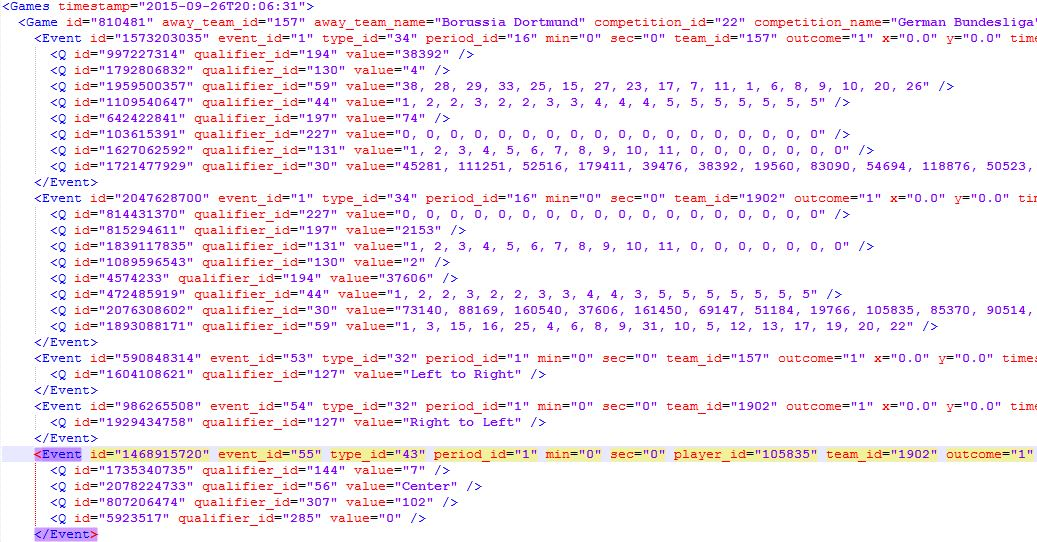
\includegraphics[scale=0.52]{se-wa-jpg/daten}
\caption{Auszug aus der XML-Datei mit den Events}
\label{xmldaten}
\end{figure}

Die \vref{xmldaten} zeigt einen Ausschnitt aus der XML-Datei in der alle Events eines Spiels aufzeichnet sind. Im oberen Teil sind die Mannschaftsaufstellungen zu sehen, wobei jeder Spieler eine eigene ID besitzt. Darunter folgt gelb markiert zum Anpfiff der Partie der erste Pass mit dem \textit{Outcome} 1, welcher einen erfolgreichen Pass identifiziert. 

\begin{sidewaysfigure}
\centering
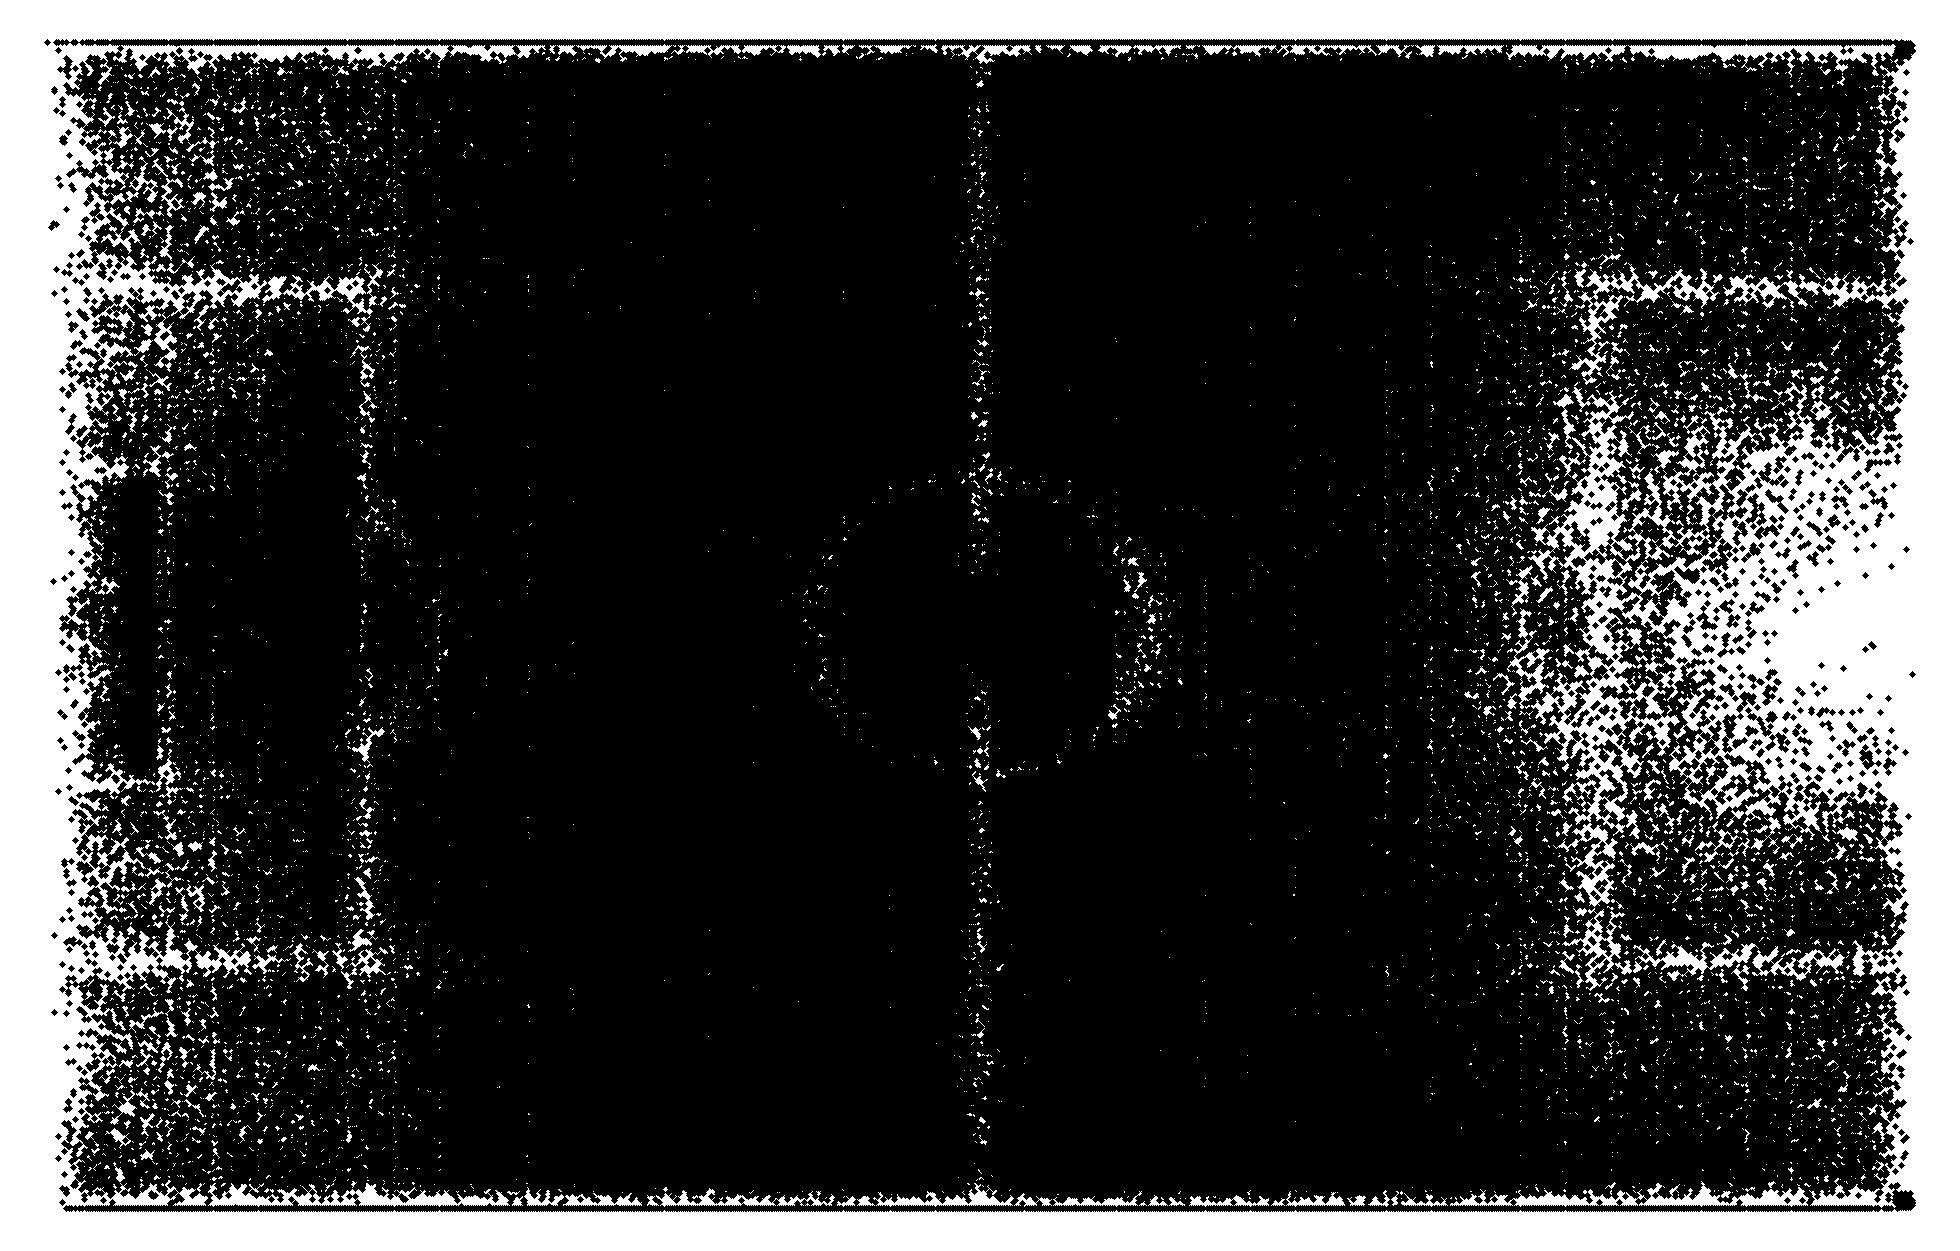
\includegraphics[scale=0.3]{se-wa-jpg/lines}
\caption[Problem der weißen Linien]{Problem der weißen Linien}
\label{lines}
\end{sidewaysfigure}

\chapter{MATLAB}

\begin{figure}[H]
\centering
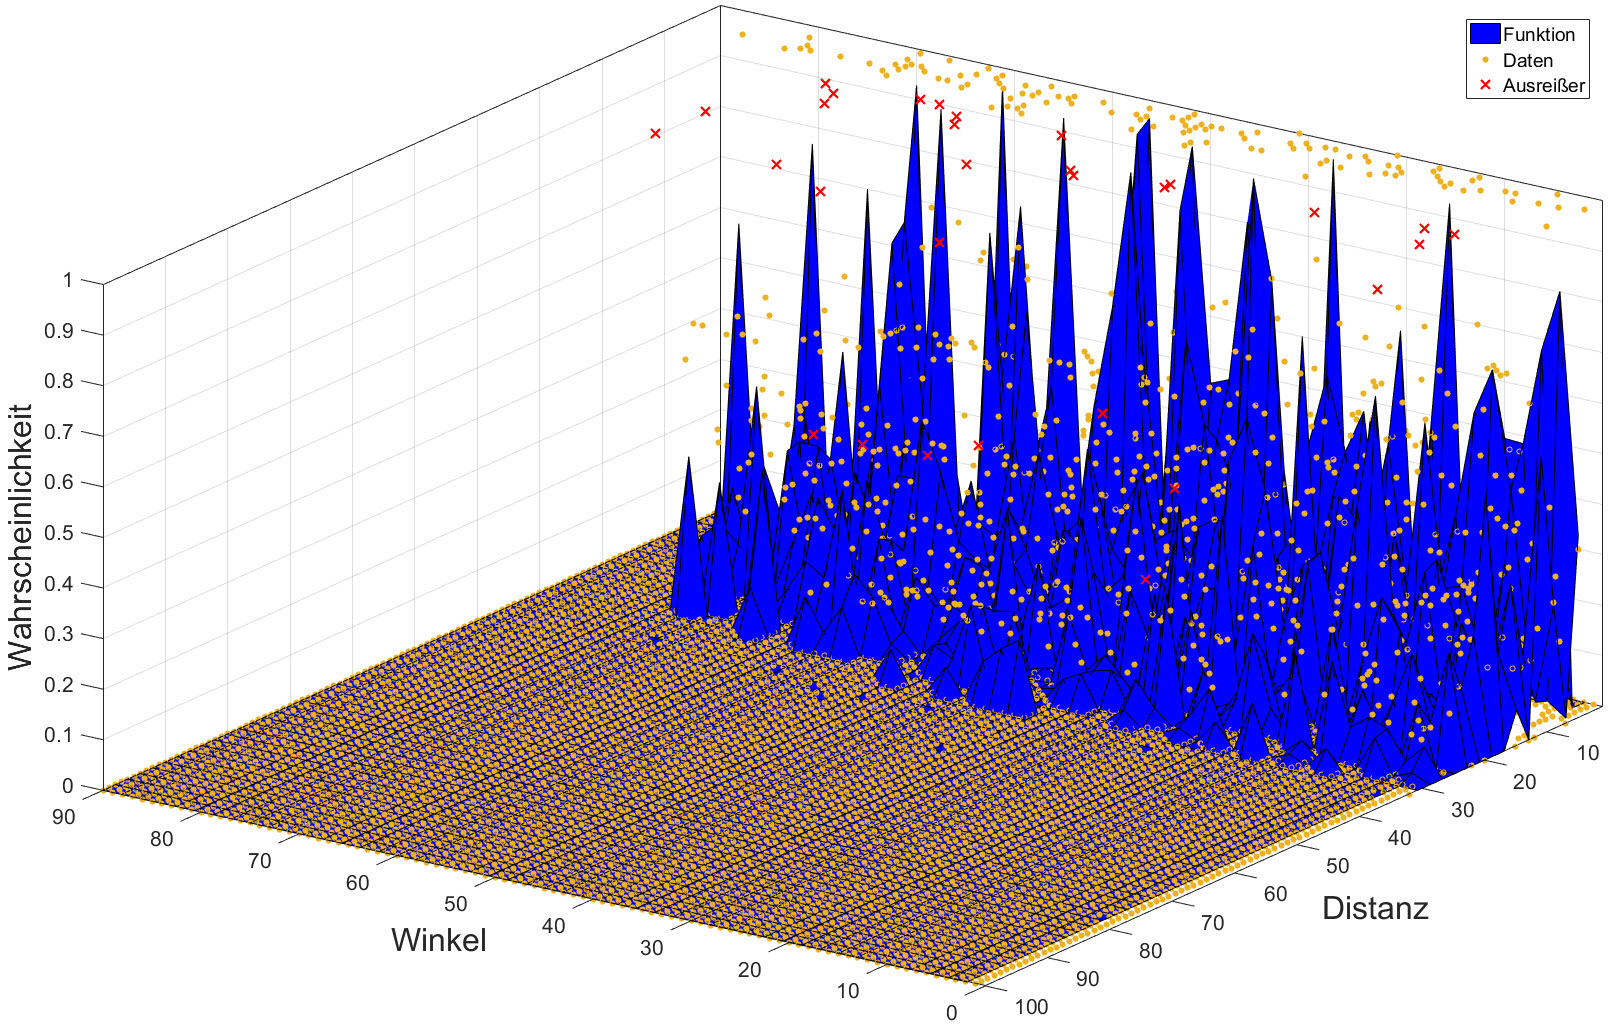
\includegraphics[scale=0.34]{se-wa-jpg/inter}
\caption{Ausschluss der Interpolation}
\label{inter}
\end{figure}

\begin{figure}[H]
\centering
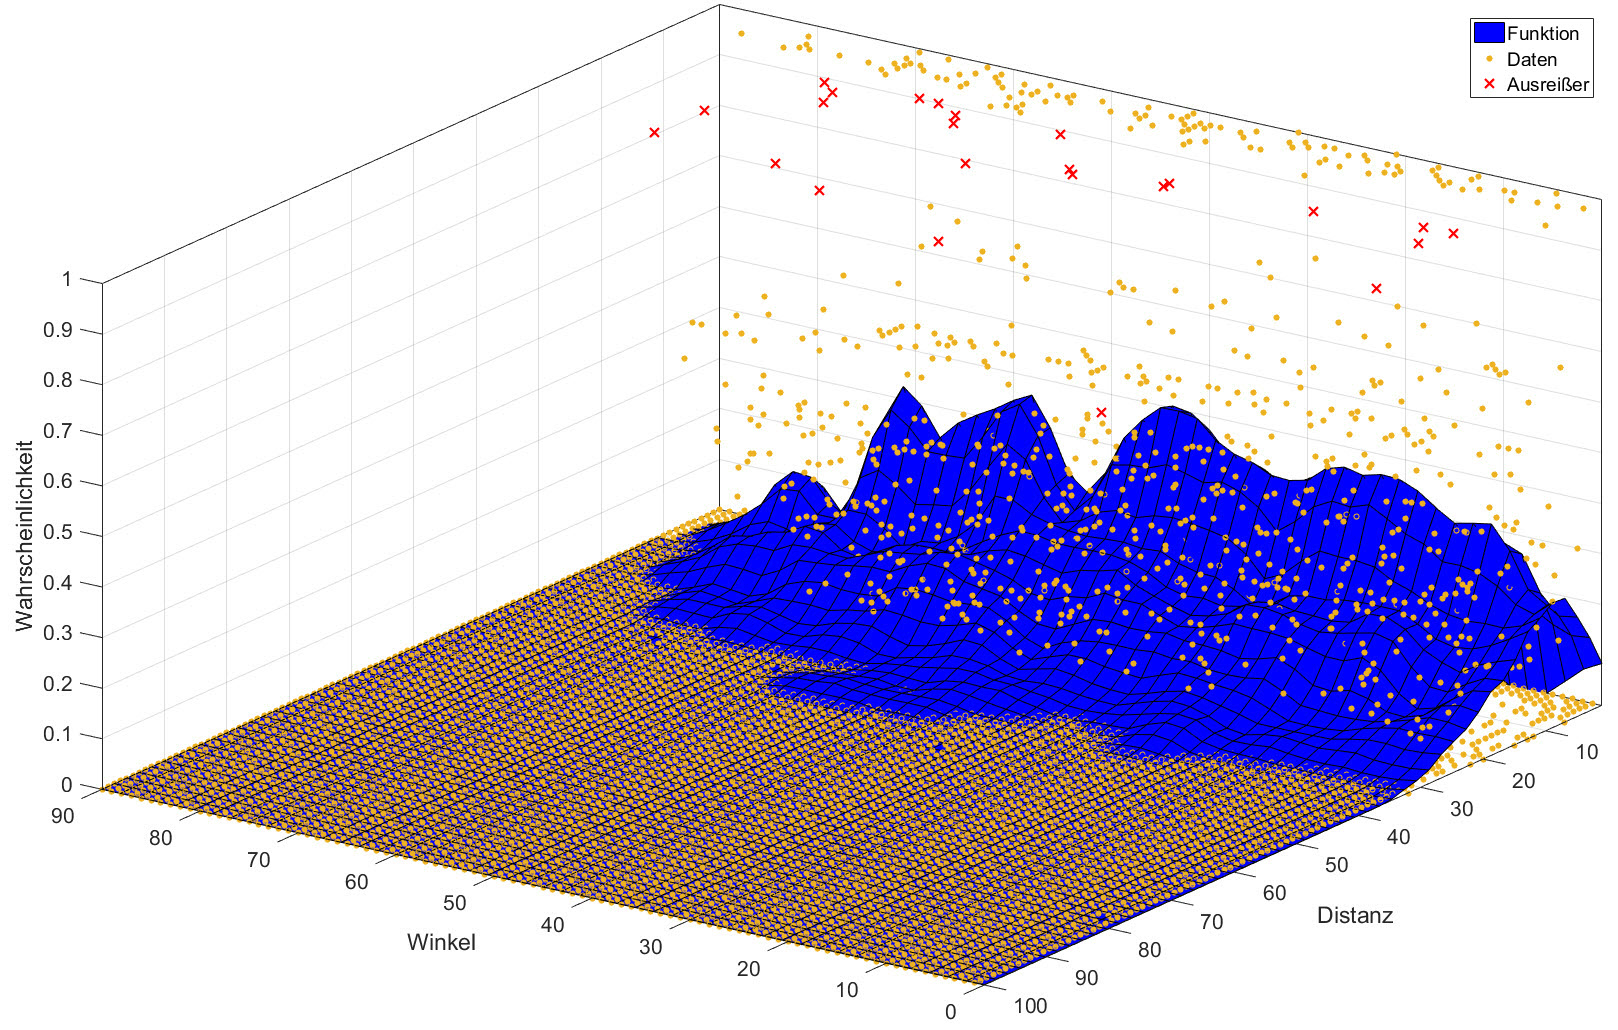
\includegraphics[scale=0.34]{se-wa-jpg/splinewdTM}
\caption{Overfitting bei einem Span-Wert von 1\%}
\label{splinewdTM}
\end{figure}

\begin{figure}[H]
\centering
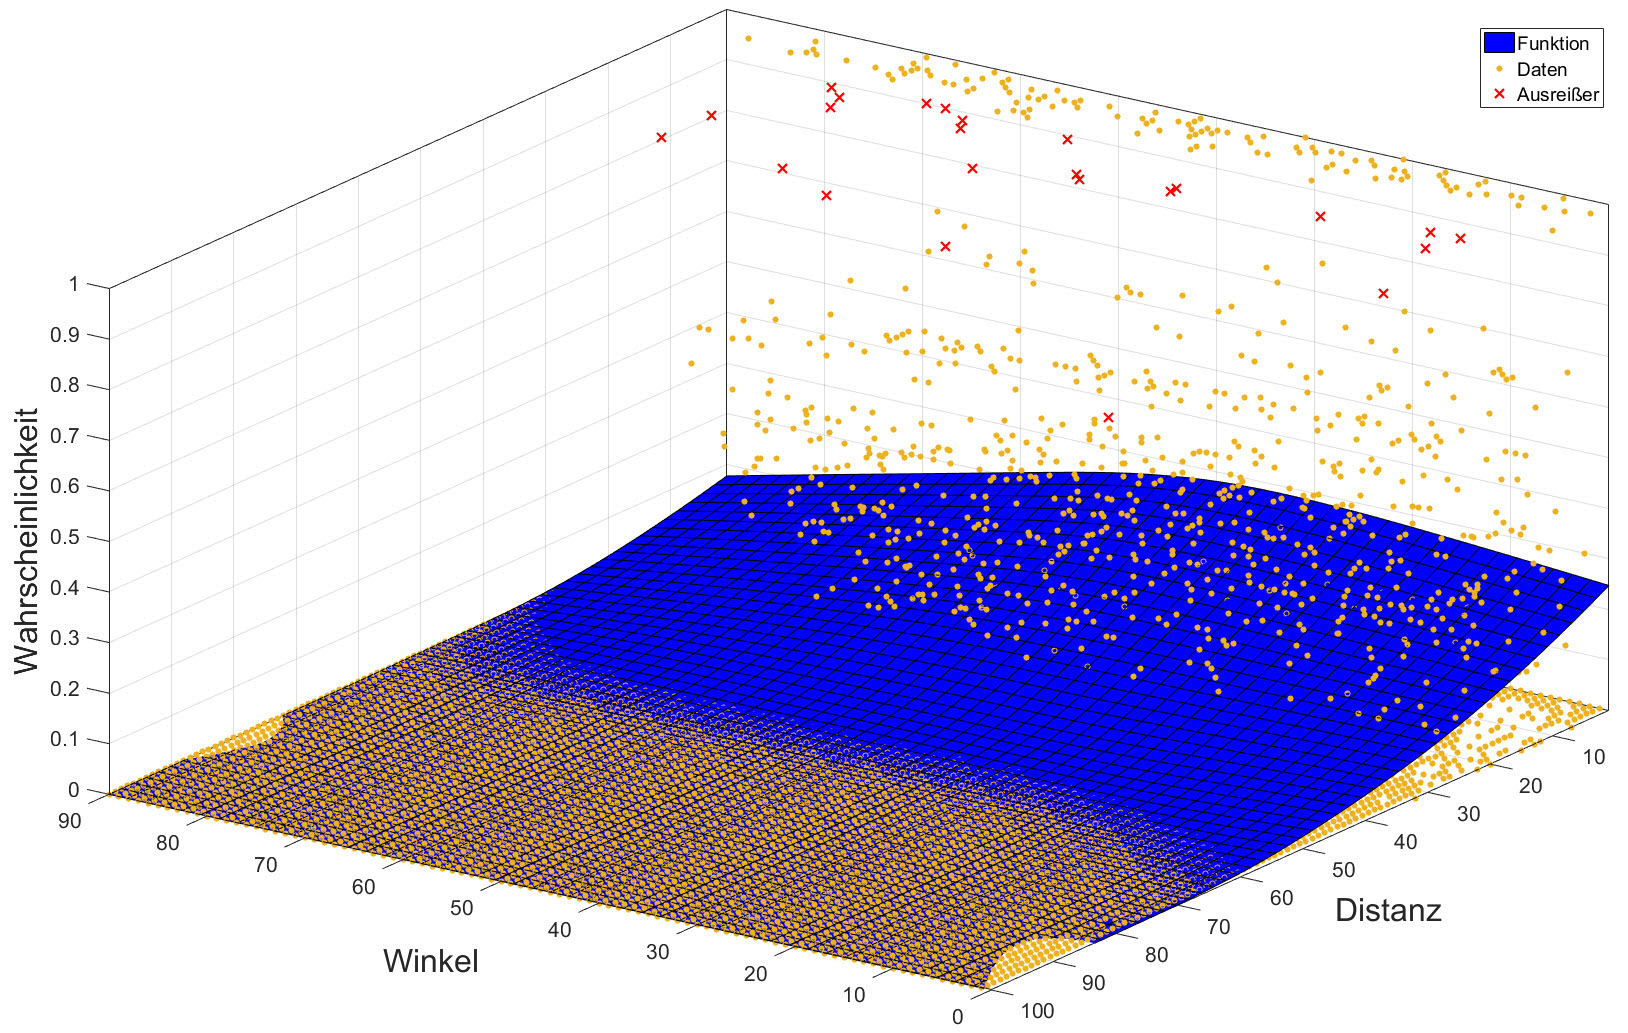
\includegraphics[scale=0.34]{se-wa-jpg/splinewdTL}
\caption{Underfitting bei einem Span-Wert von 50\%}
\label{splinewdTL}
\end{figure}

\chapter{Evaluation}
\label{anheva}

Hier werden die Ergebnisse der Evaluation des nichtparametrischen Regressionsmodelles unter der Betrachtung der Position des Schusses dokumentiert. Dazu wurden folgende Bundesliga-Saisons:

\begin{itemize}
\item Bundesliga-Saison 2014/2015 
\item Bundesliga-Saison 2015/2016 
\item Bundesliga-Saison 2016/2017 
\end{itemize}

unter der Betrachtung der Zusammenhänge zwischen:

\begin{itemize}
\item erwarteten Anzahl an \textbf{Gegentoren} gegenüber der tatsächlichen erhaltenen Anzahl an \textbf{Gegentoren}
\item erwarteten Anzahl an \textbf{Toren} gegenüber der tatsächlichen erzielten Anzahl an\textbf{Gegentoren}
\item erwarteten Anzahl an \textbf{Punkten} gegenüber der tatsächlichen gewonnen Anzahl an \textbf{Punkten}
\end{itemize}

evaluiert. Die Korrelationskoeffizienten geben auf einer Skala von -1 bis 1 darüber Aufschluss, wie stark der Zusammenhang zwischen den erwarteten Werten und den tatsächlichen Werten ist. Im Durchschnitt ergibt sich daraus ein Wert von \textsf{0.81}, welcher für einen starken Zusammenhang und damit für eine gute Anpassung des Modelles an die Daten spricht.


\begin{sidewaysfigure}
\centering
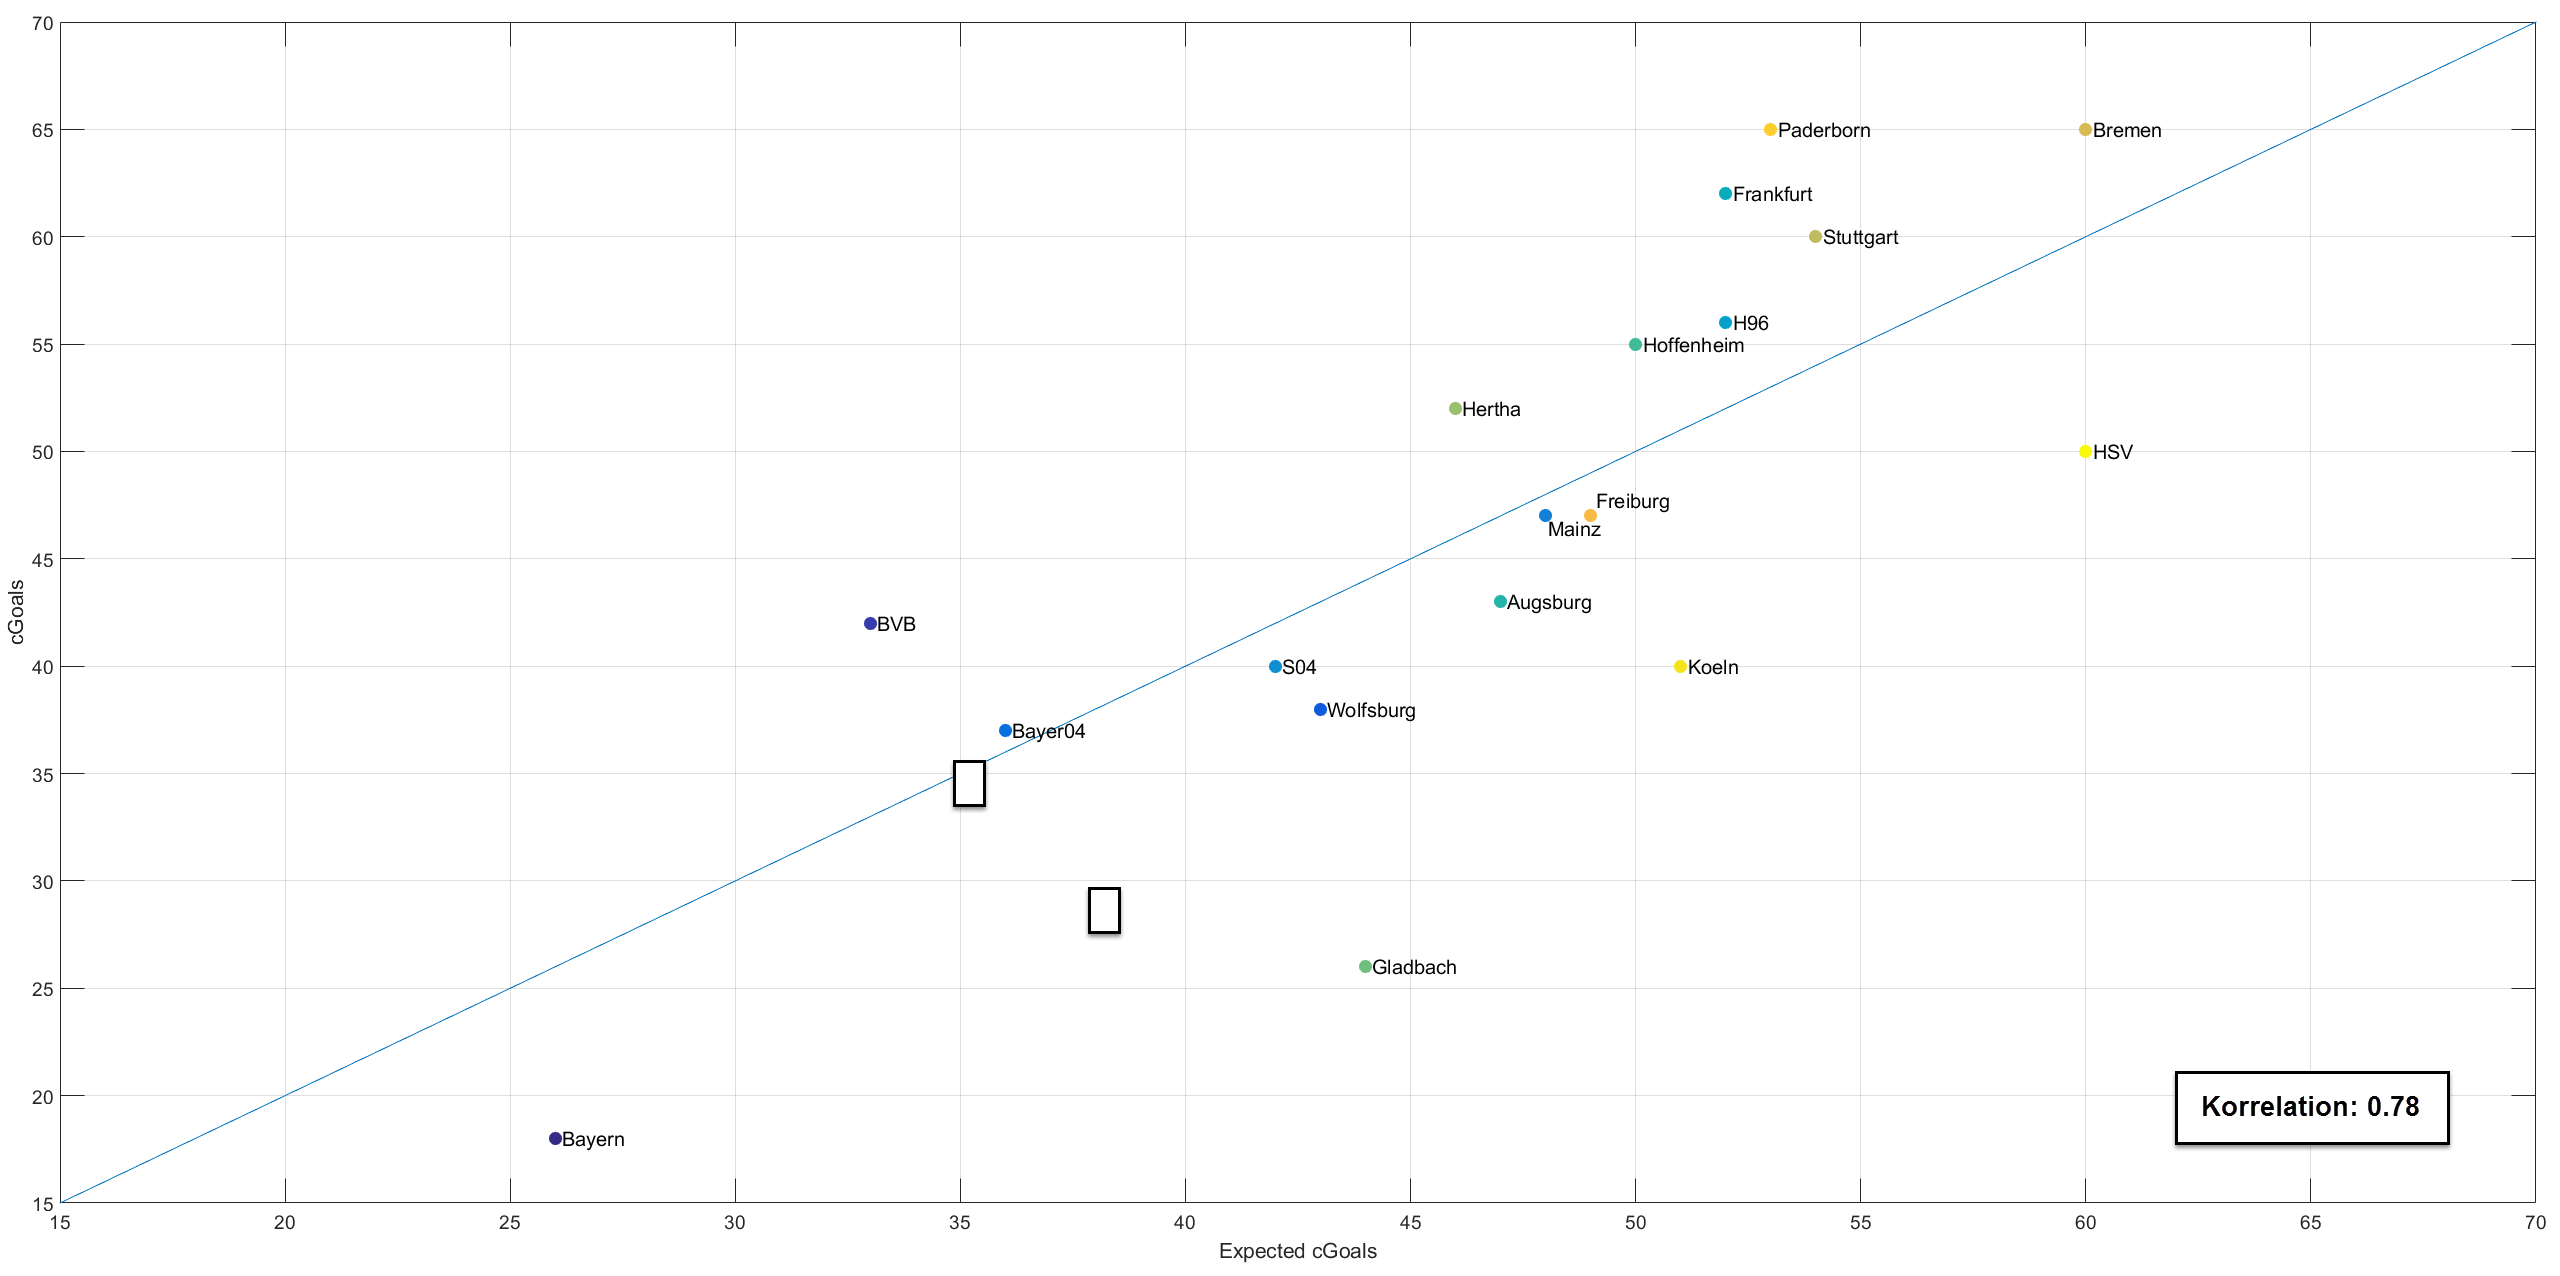
\includegraphics[scale=0.3]{se-wa-jpg/cGoals_correlation_14_15}
\caption{Evaluation der Gegentore der Saison 2014/15}
\label{cg1415}
\end{sidewaysfigure}

\begin{sidewaysfigure}
\centering
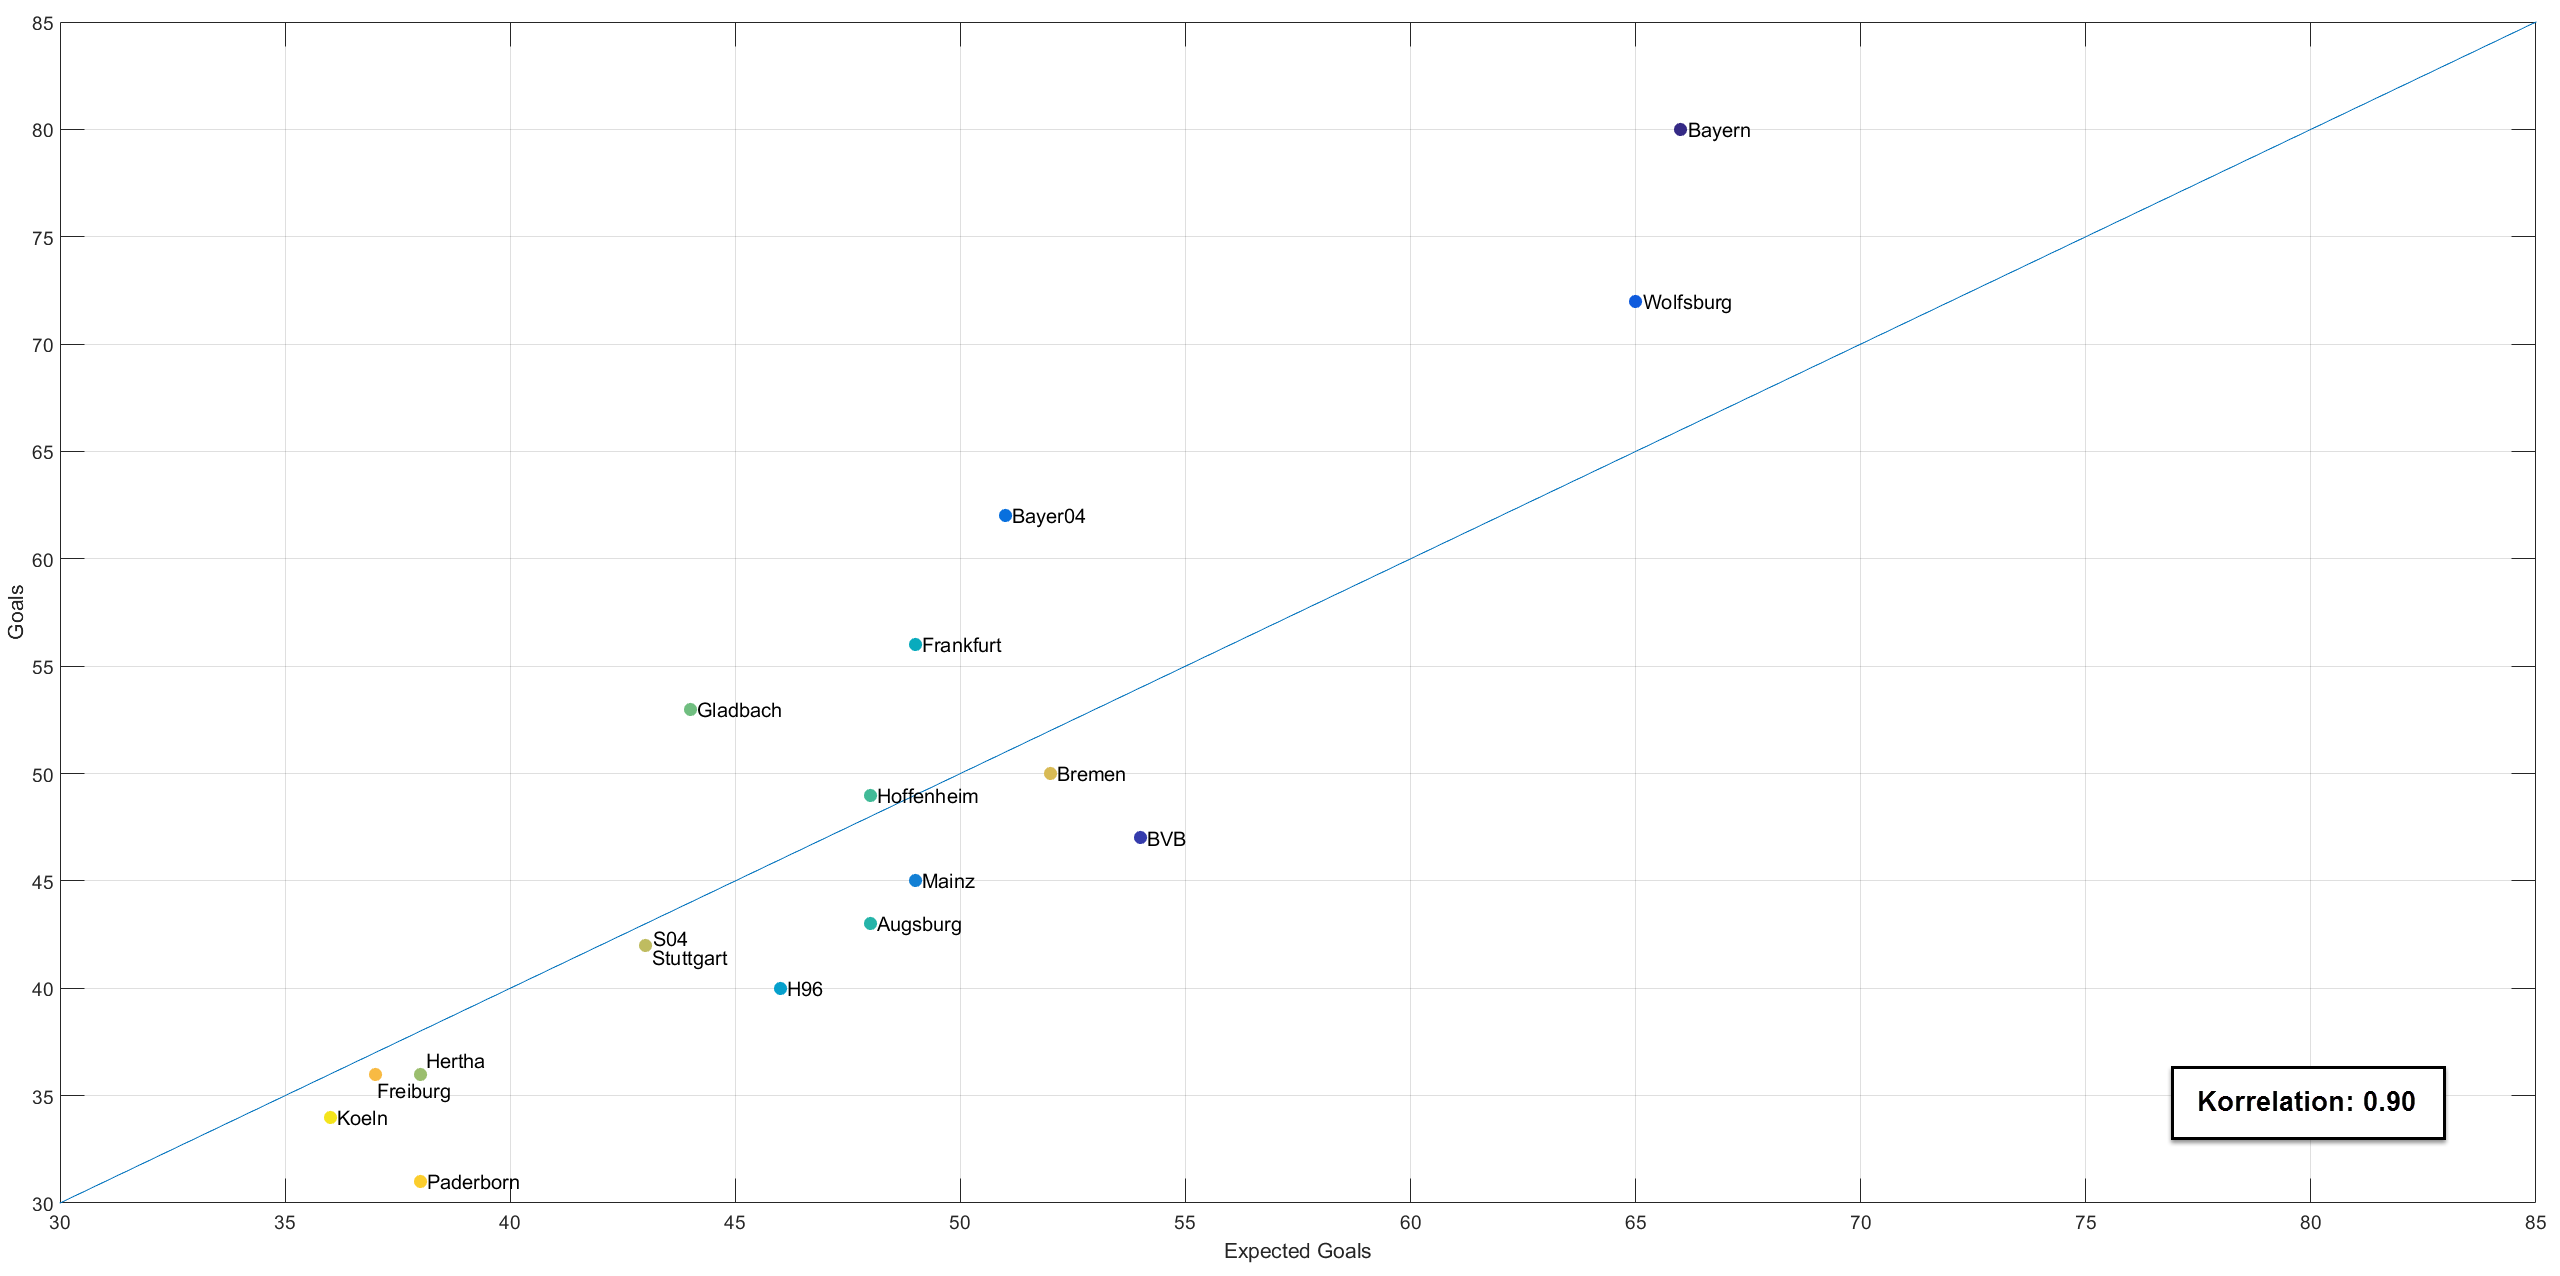
\includegraphics[scale=0.3]{se-wa-jpg/goals_correlation_14_15}
\caption{Evaluation der Tore der Saison 2014/15}
\label{g1415}
\end{sidewaysfigure}

\begin{sidewaysfigure}
\centering
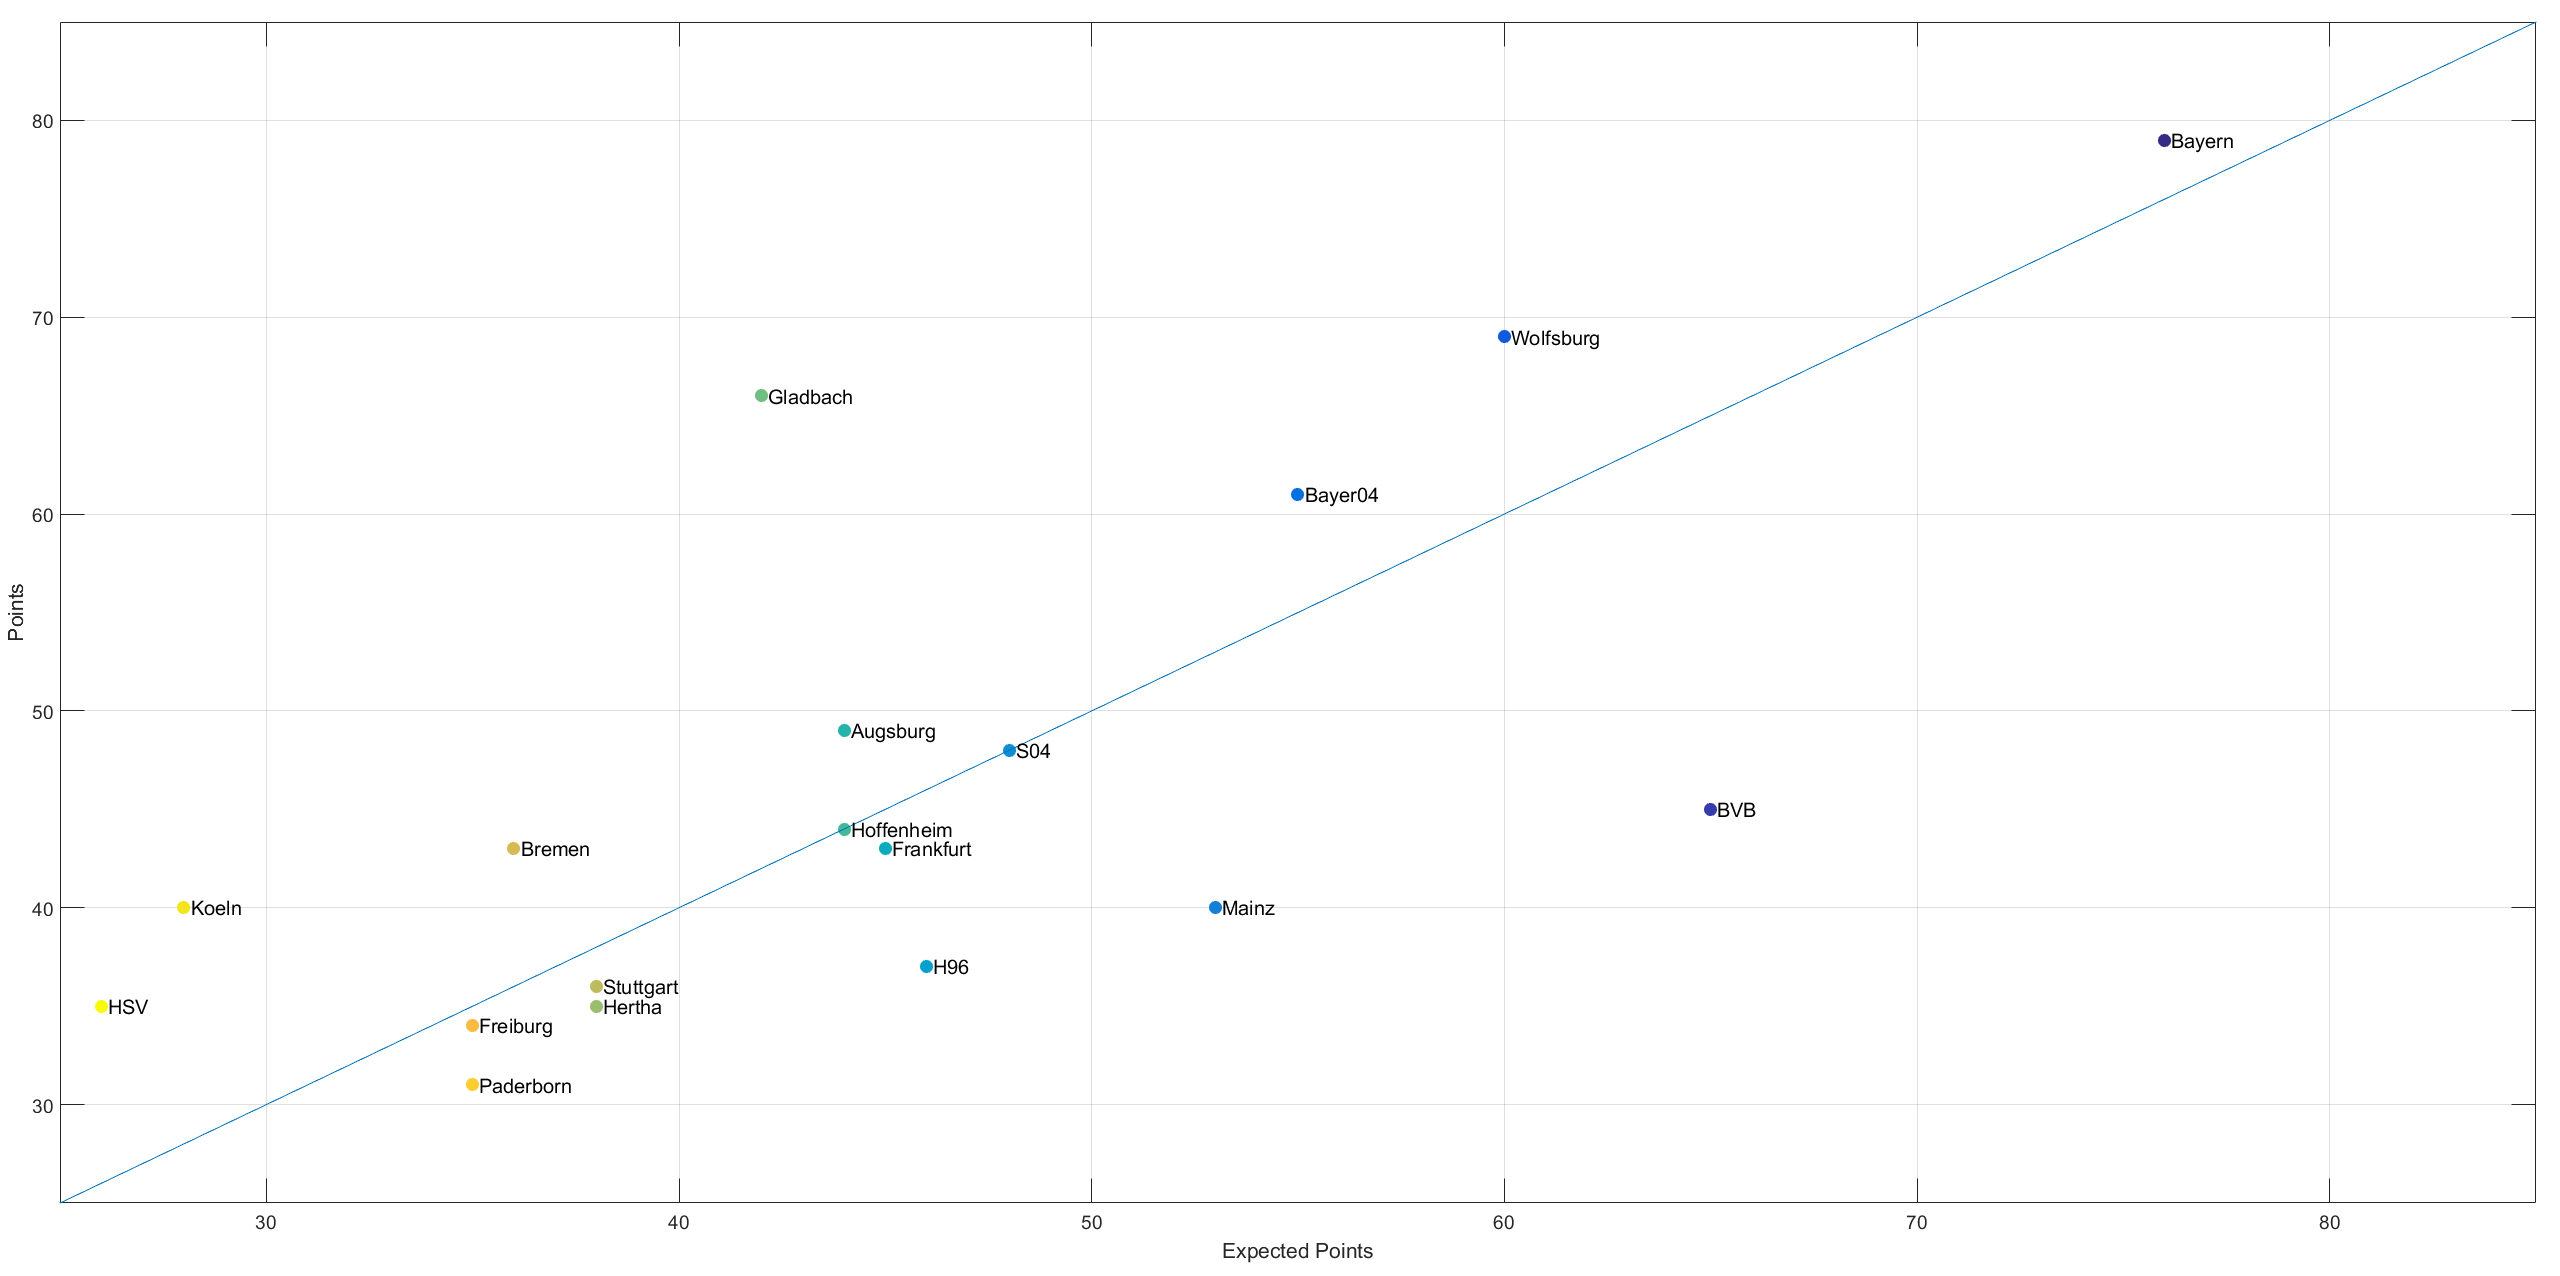
\includegraphics[scale=0.3]{se-wa-jpg/points_correlation_14_15}
\caption{Evaluation der Punkte der Saison 2014/15}
\label{p1415}
\end{sidewaysfigure}

\begin{sidewaysfigure}
\centering
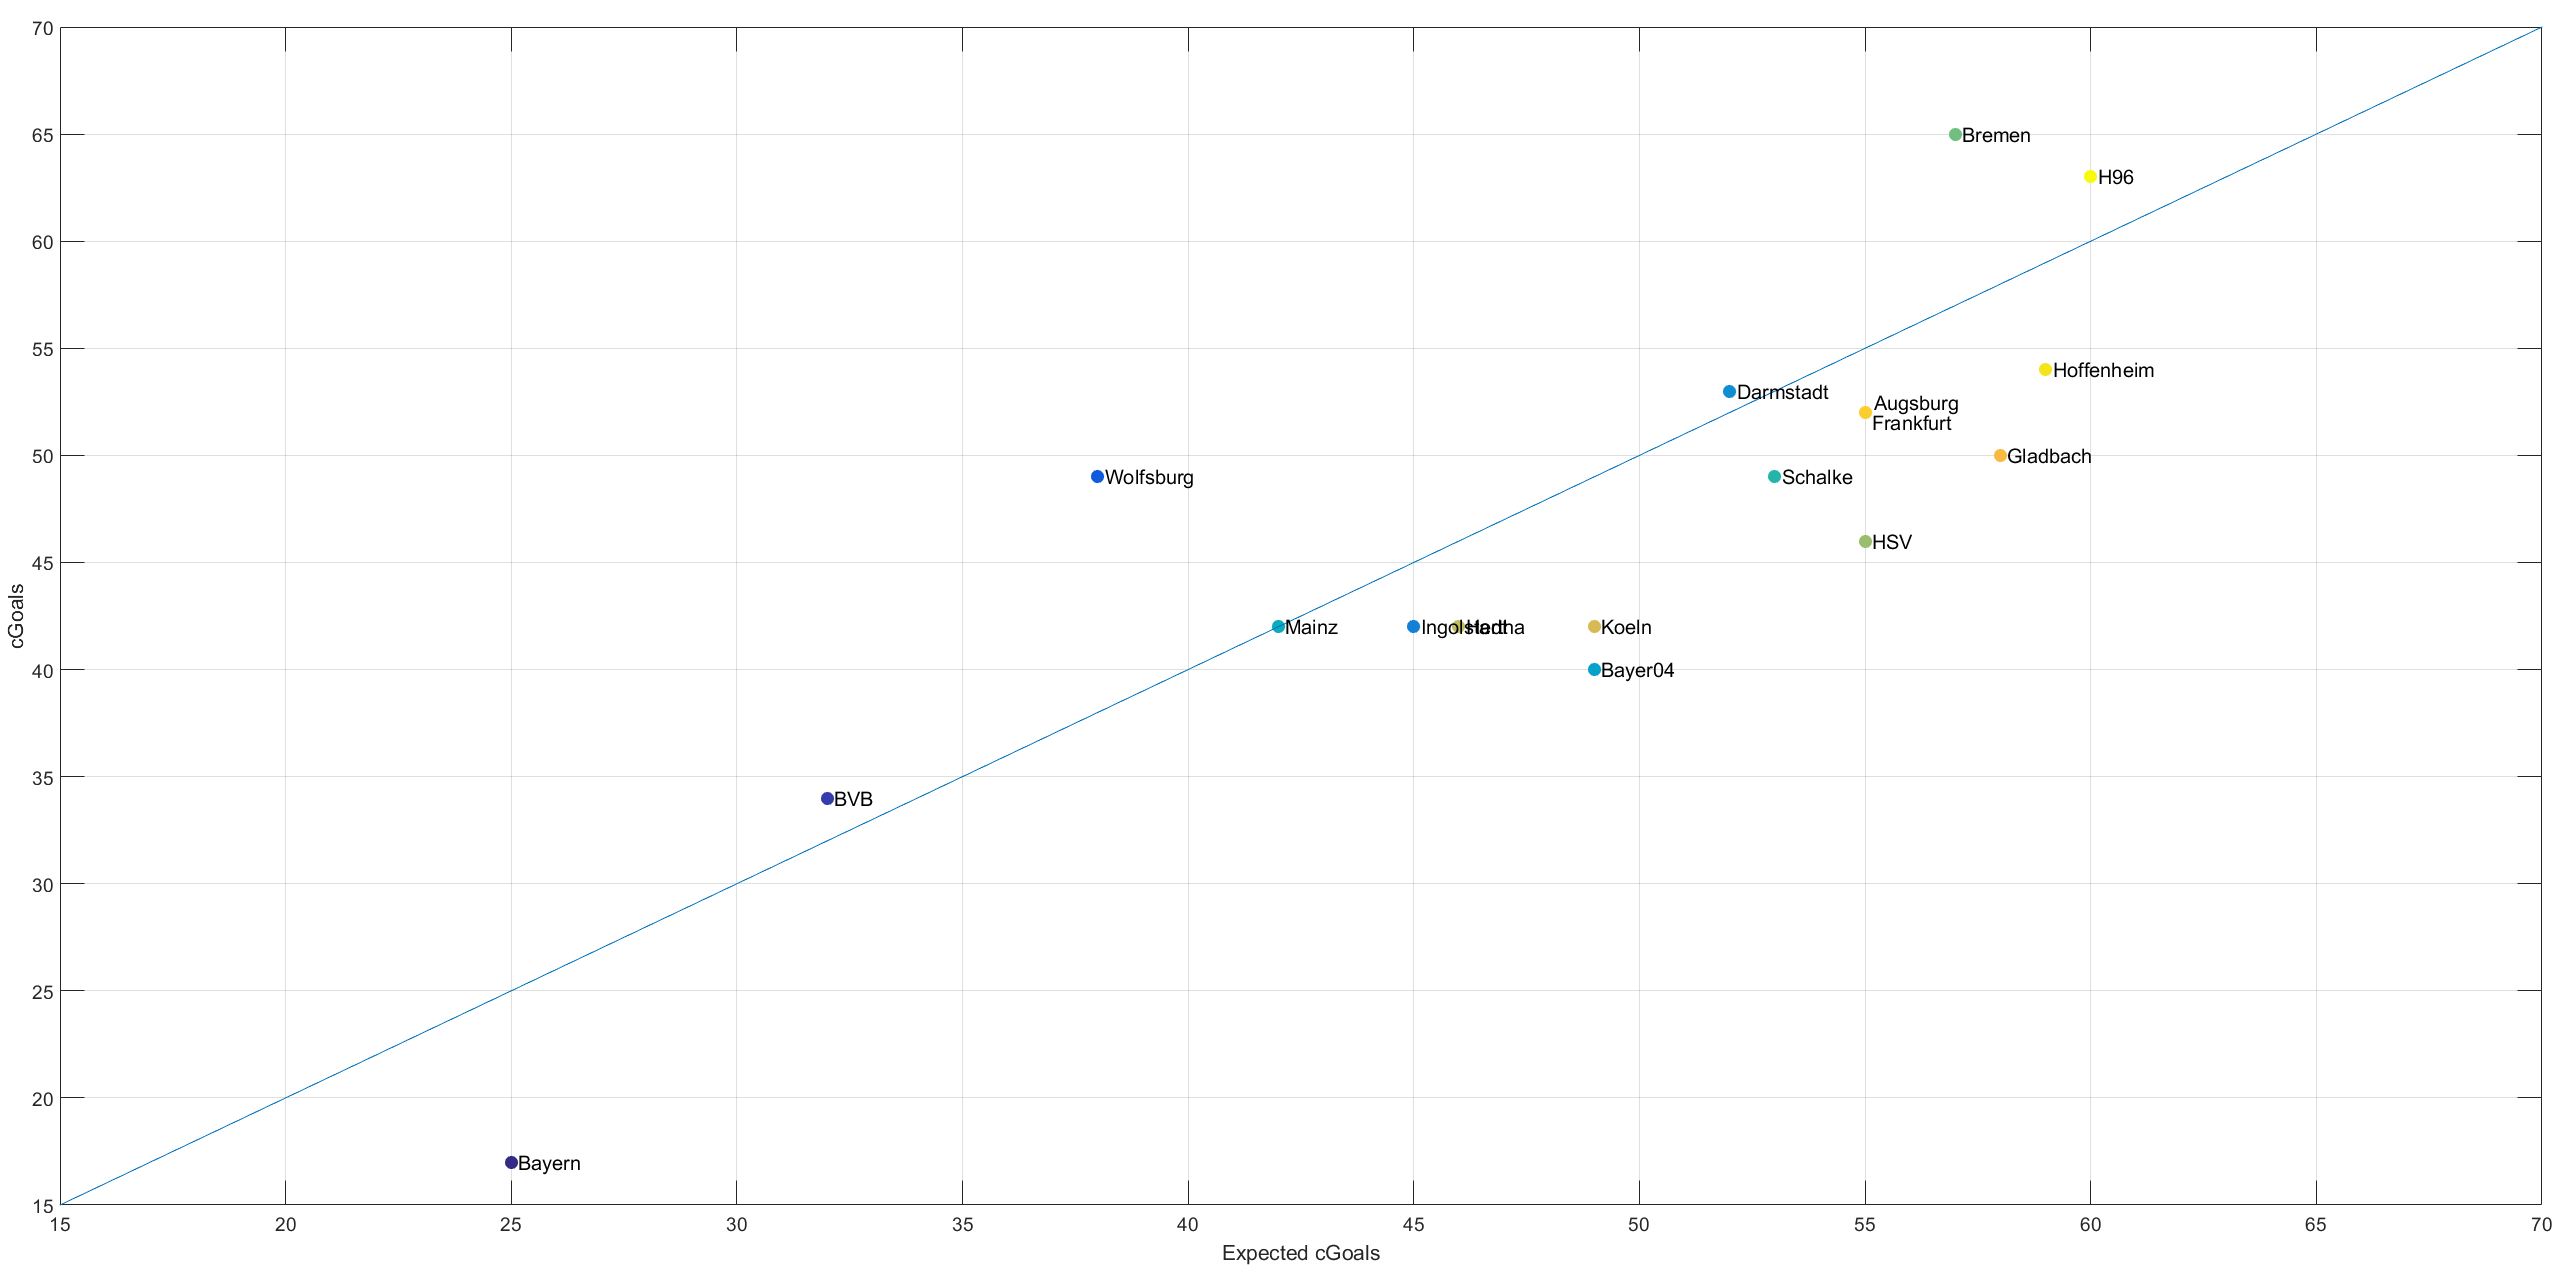
\includegraphics[scale=0.3]{se-wa-jpg/cGoals_correlation_15_16}
\caption{Evaluation der Gegentore der Saison 2015/16}
\label{lines}
\end{sidewaysfigure}

\begin{sidewaysfigure}
\centering
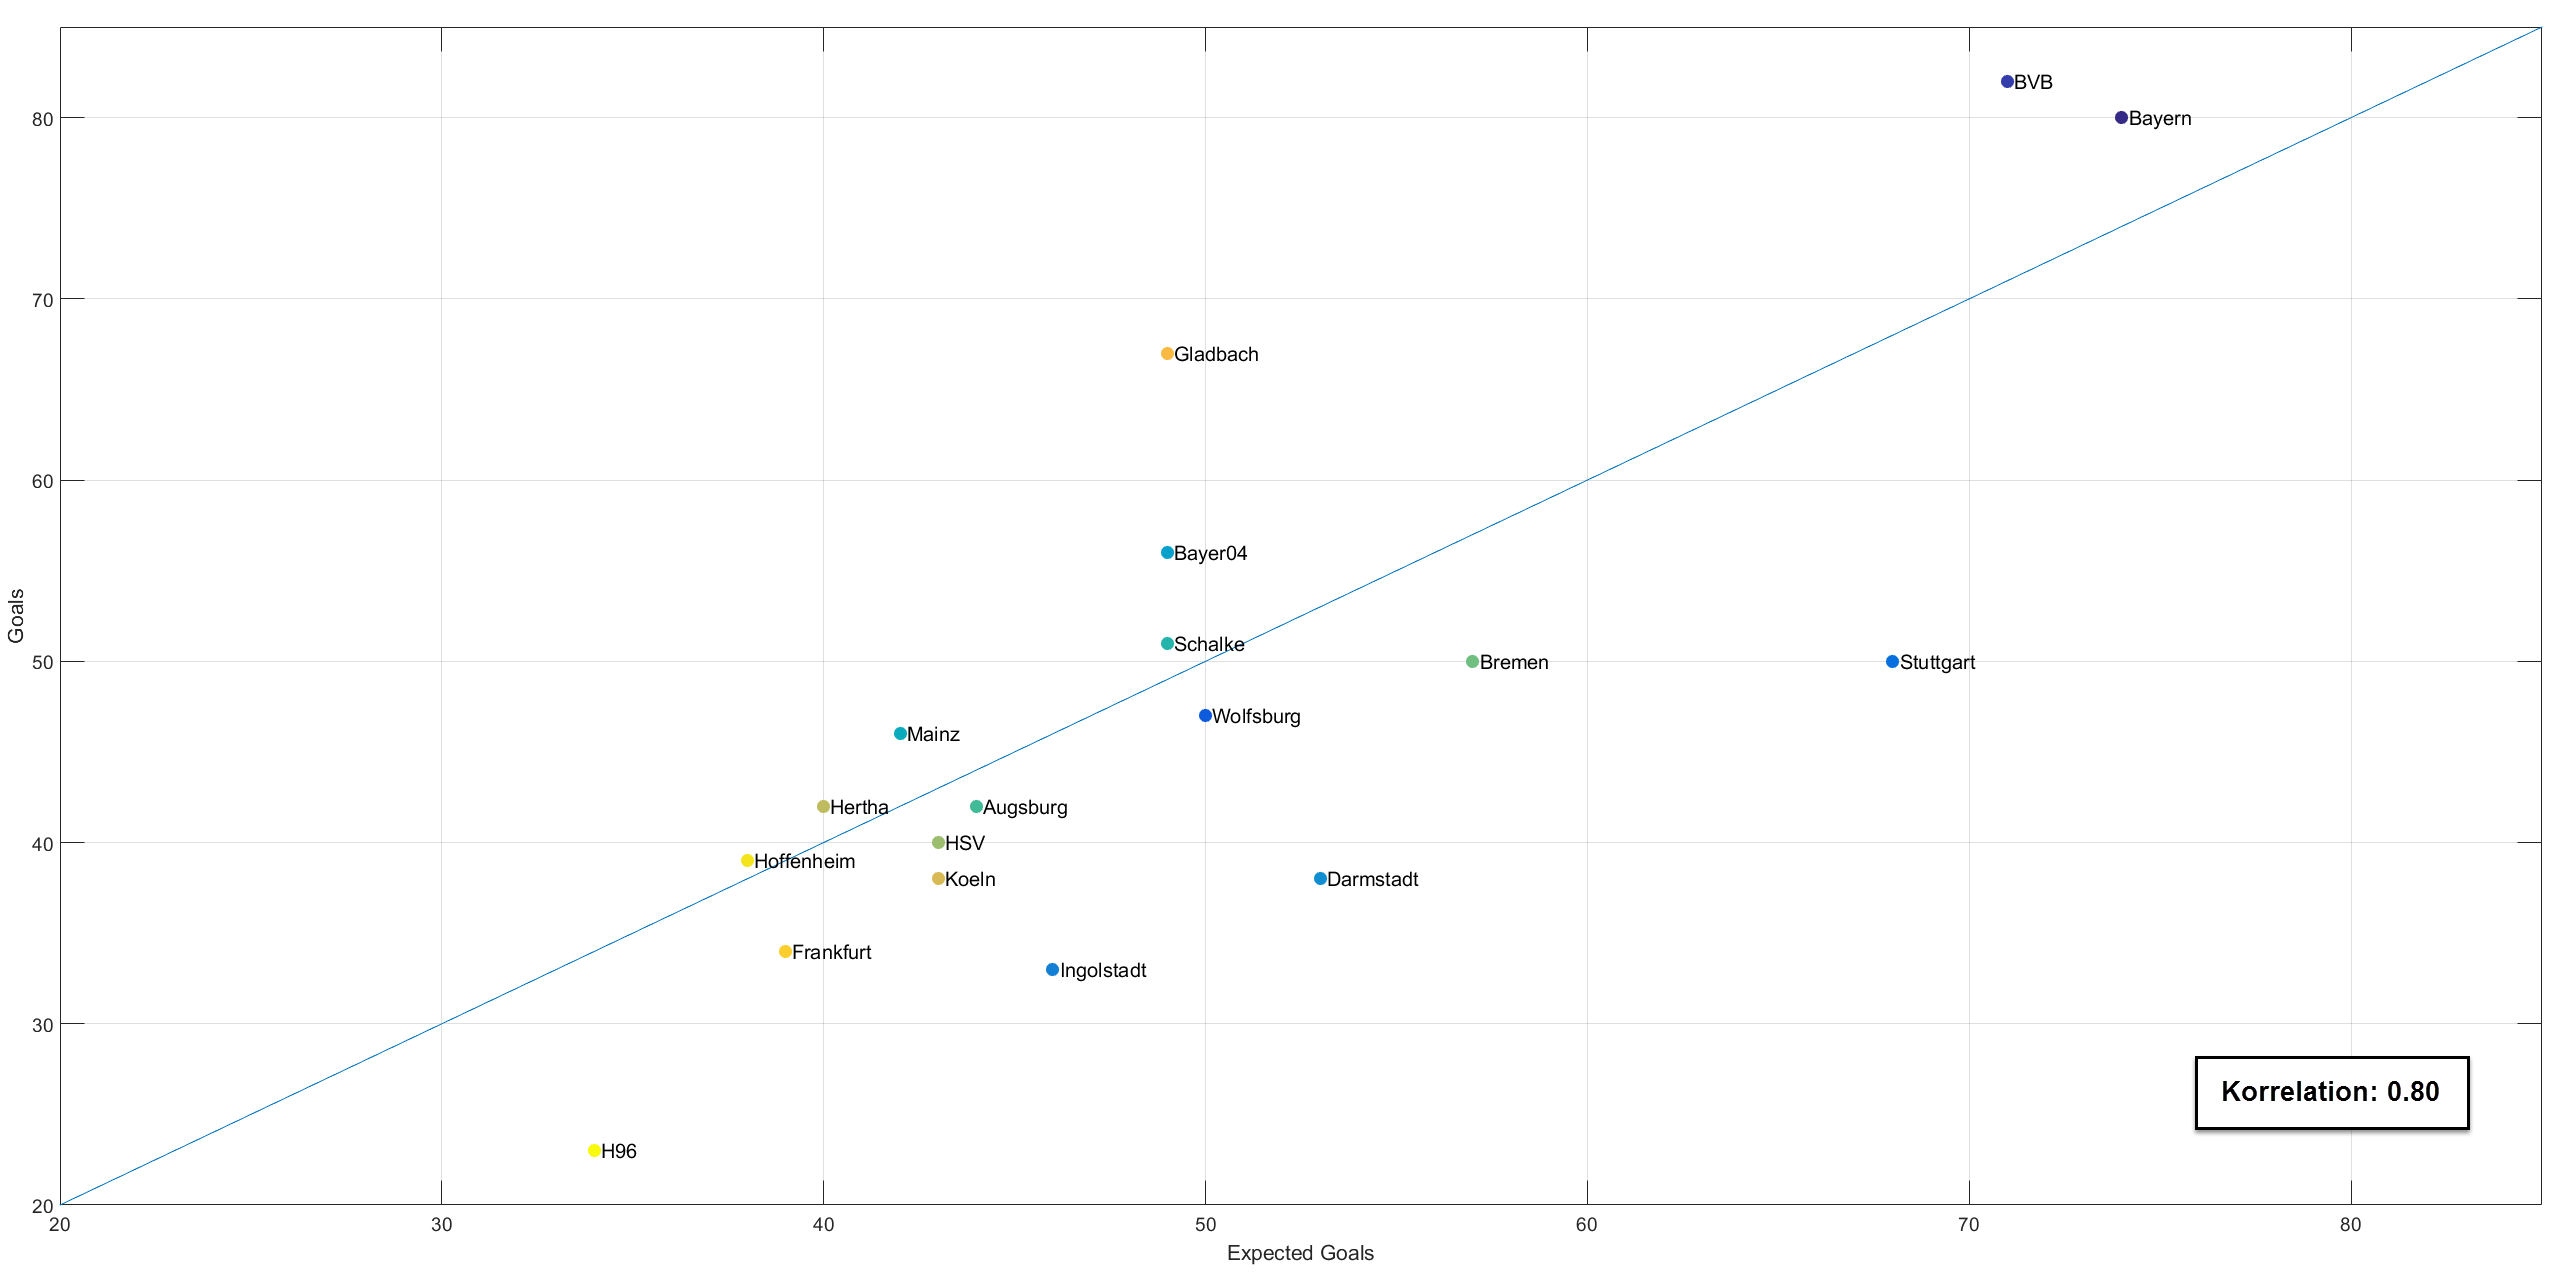
\includegraphics[scale=0.3]{se-wa-jpg/goals_correlation_15_16}
\caption{Evaluation der Tore der Saison 2015/16}
\label{lines}
\end{sidewaysfigure}

\begin{sidewaysfigure}
\centering
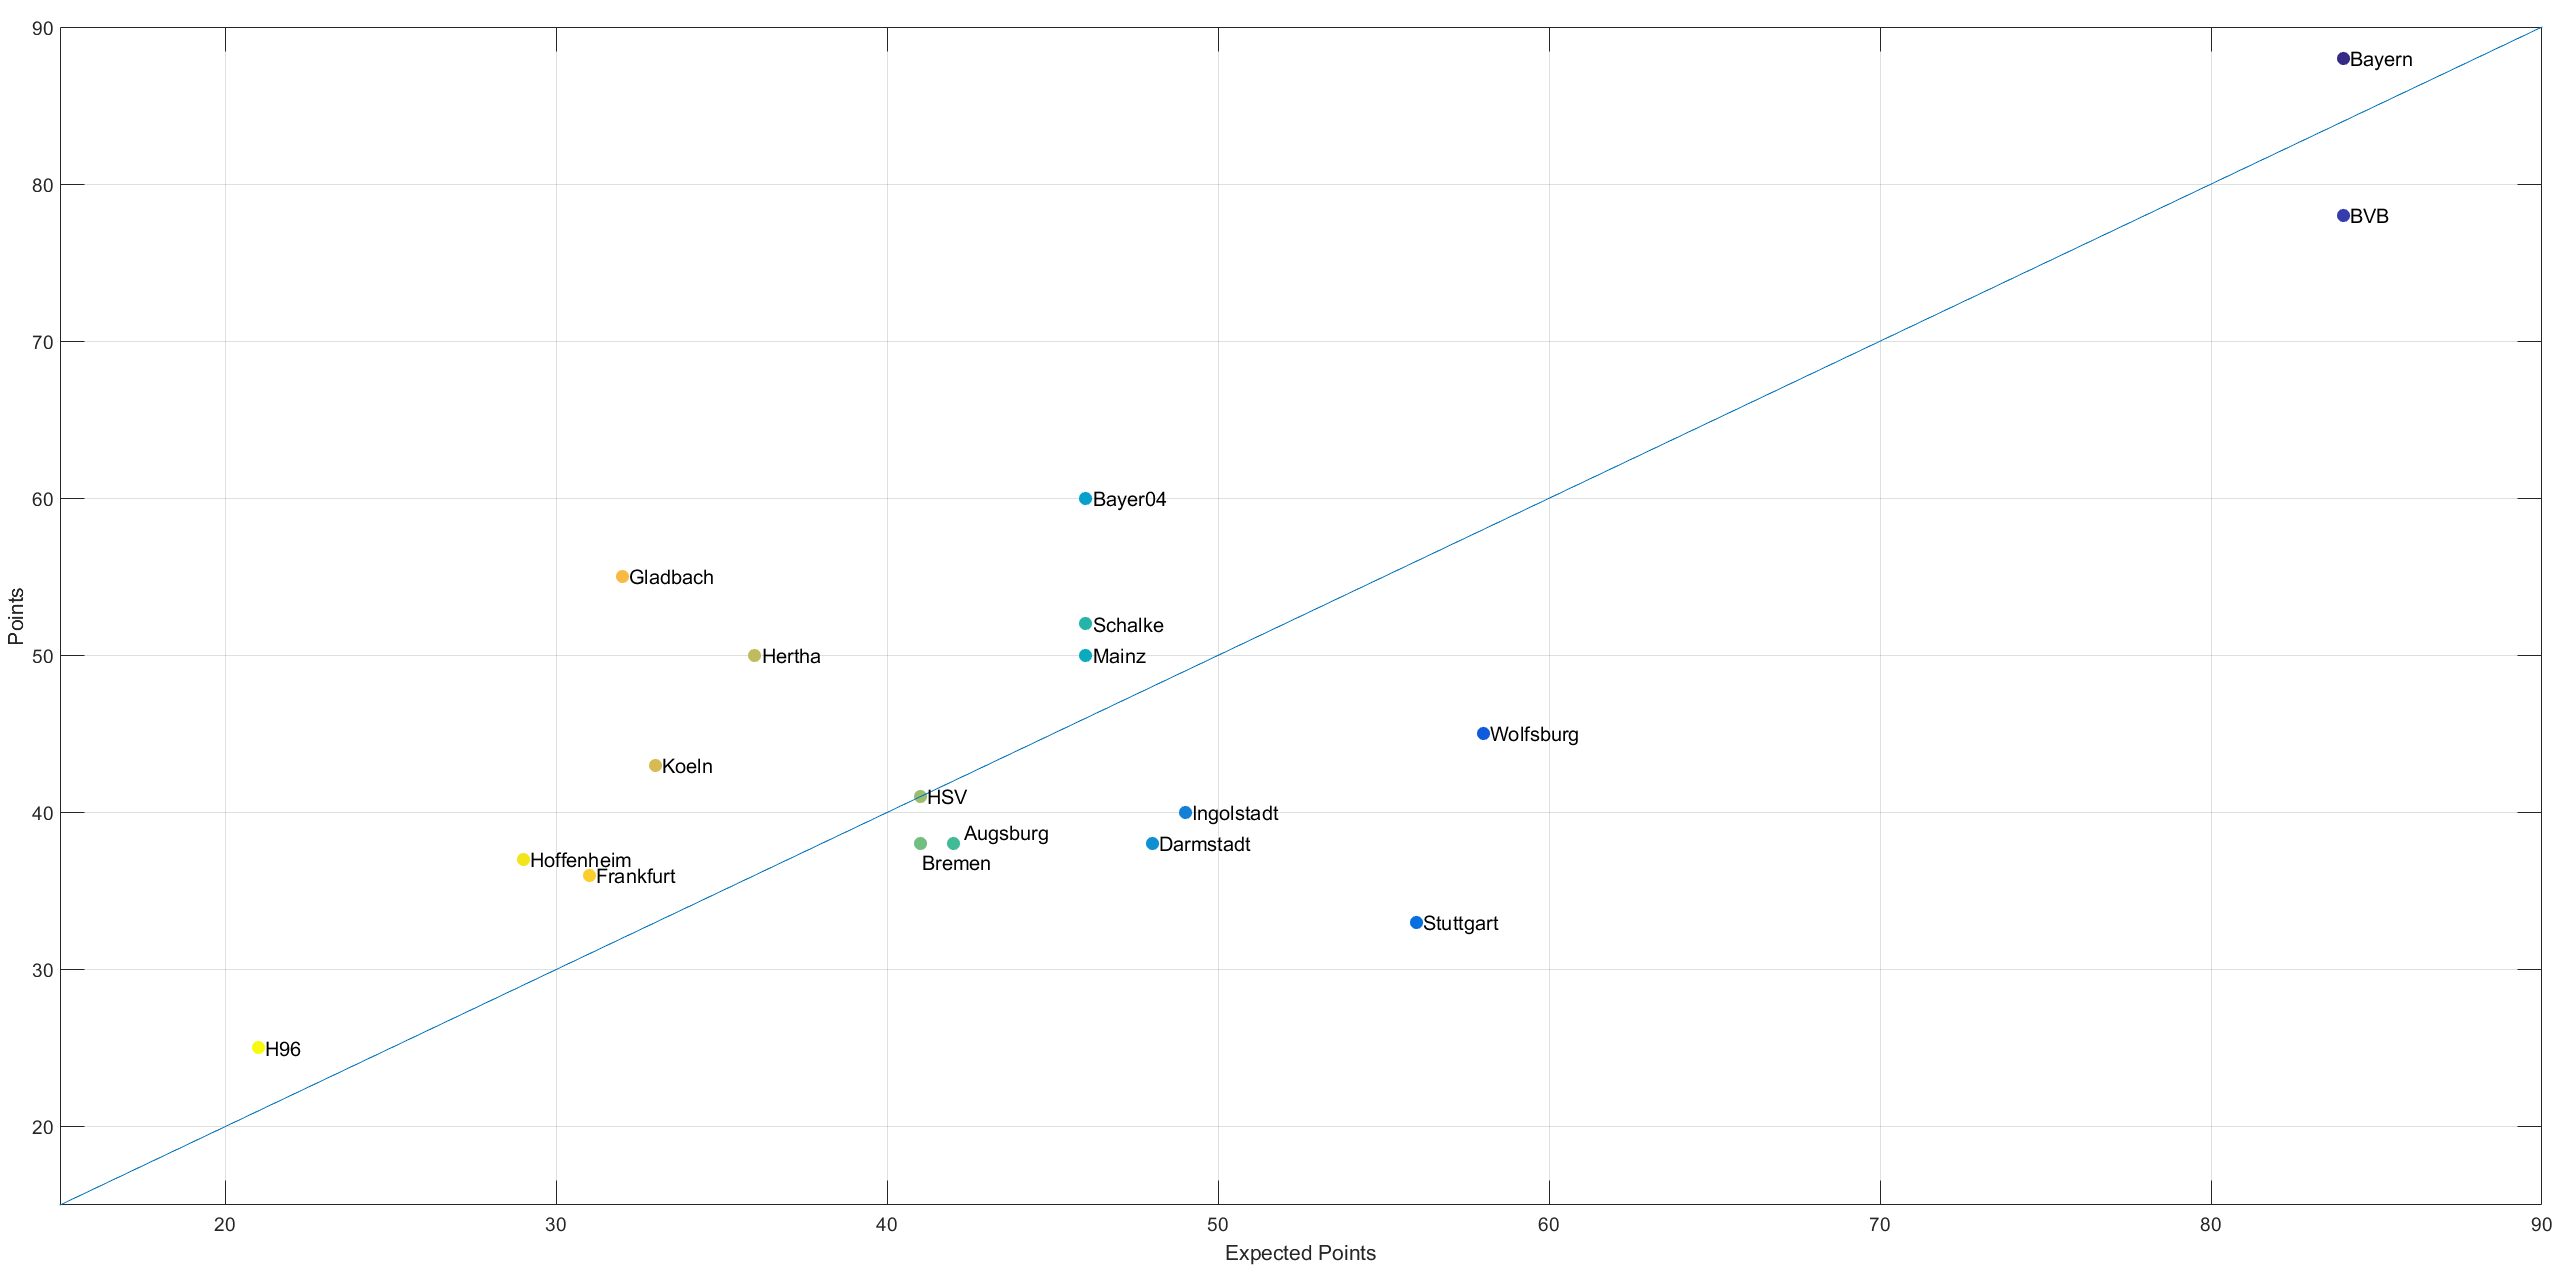
\includegraphics[scale=0.3]{se-wa-jpg/points_correlation_15_16}
\caption{Evaluation der Punkte der Saison 2015/16}
\label{lines}
\end{sidewaysfigure}

\begin{sidewaysfigure}
\centering
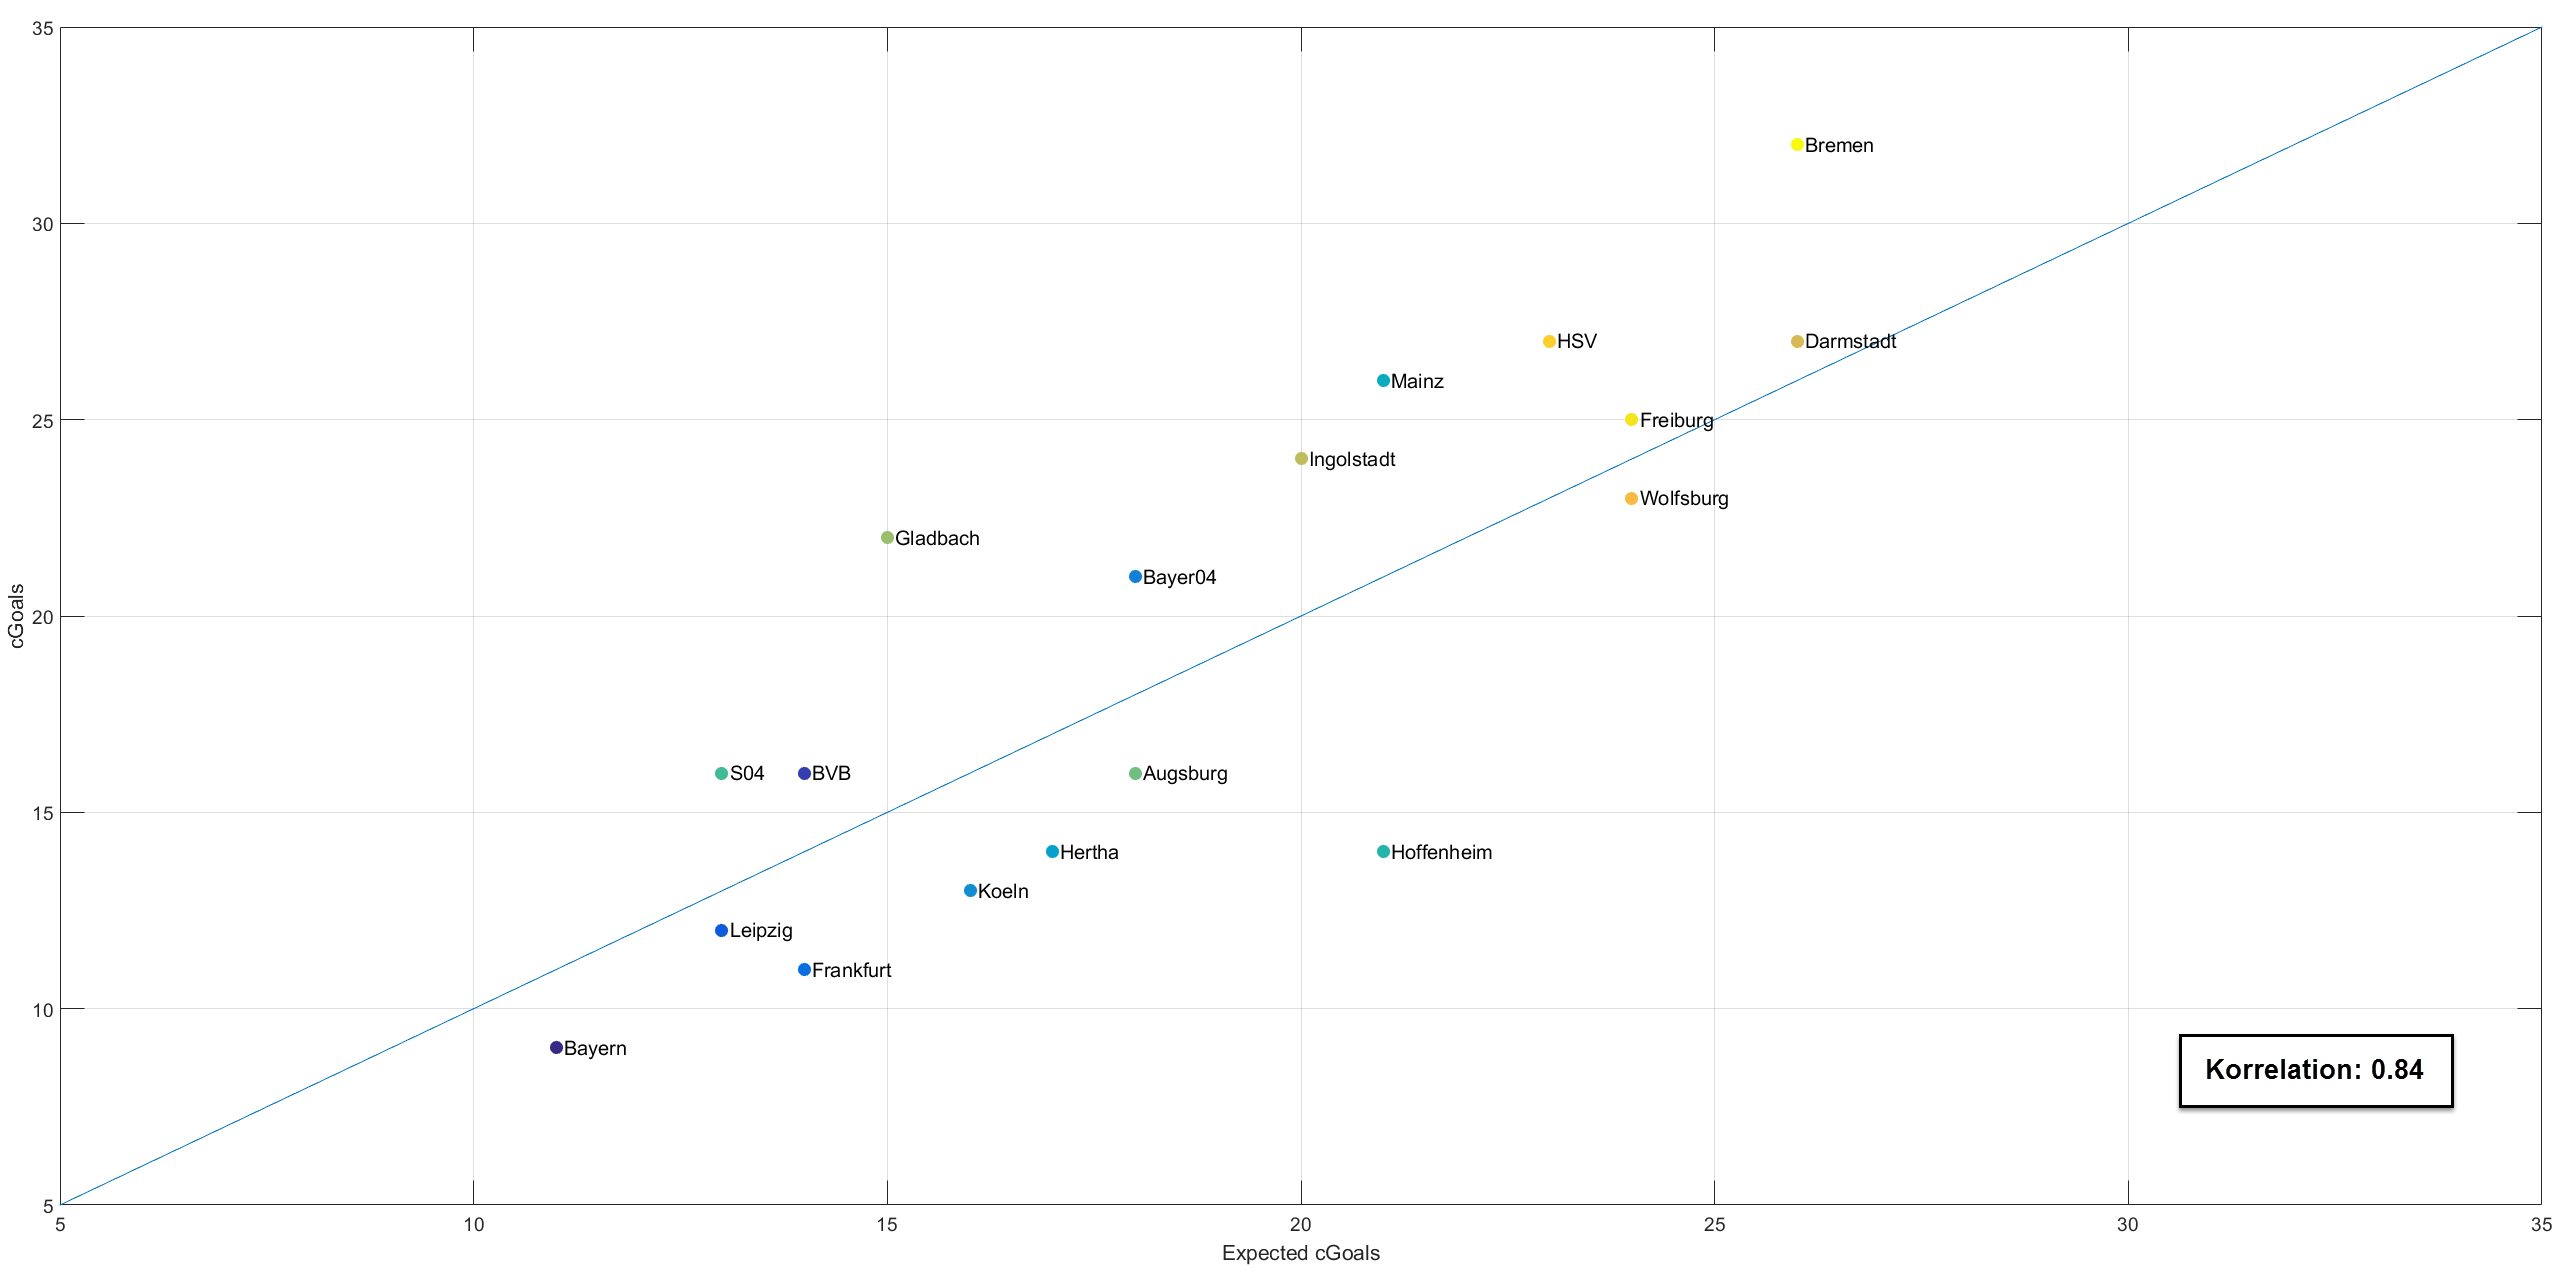
\includegraphics[scale=0.3]{se-wa-jpg/cGoals_correlation_16_17}
\caption{Evaluation der Gegentore der Saison 2016/17}
\label{lines}
\end{sidewaysfigure}

\begin{sidewaysfigure}
\centering
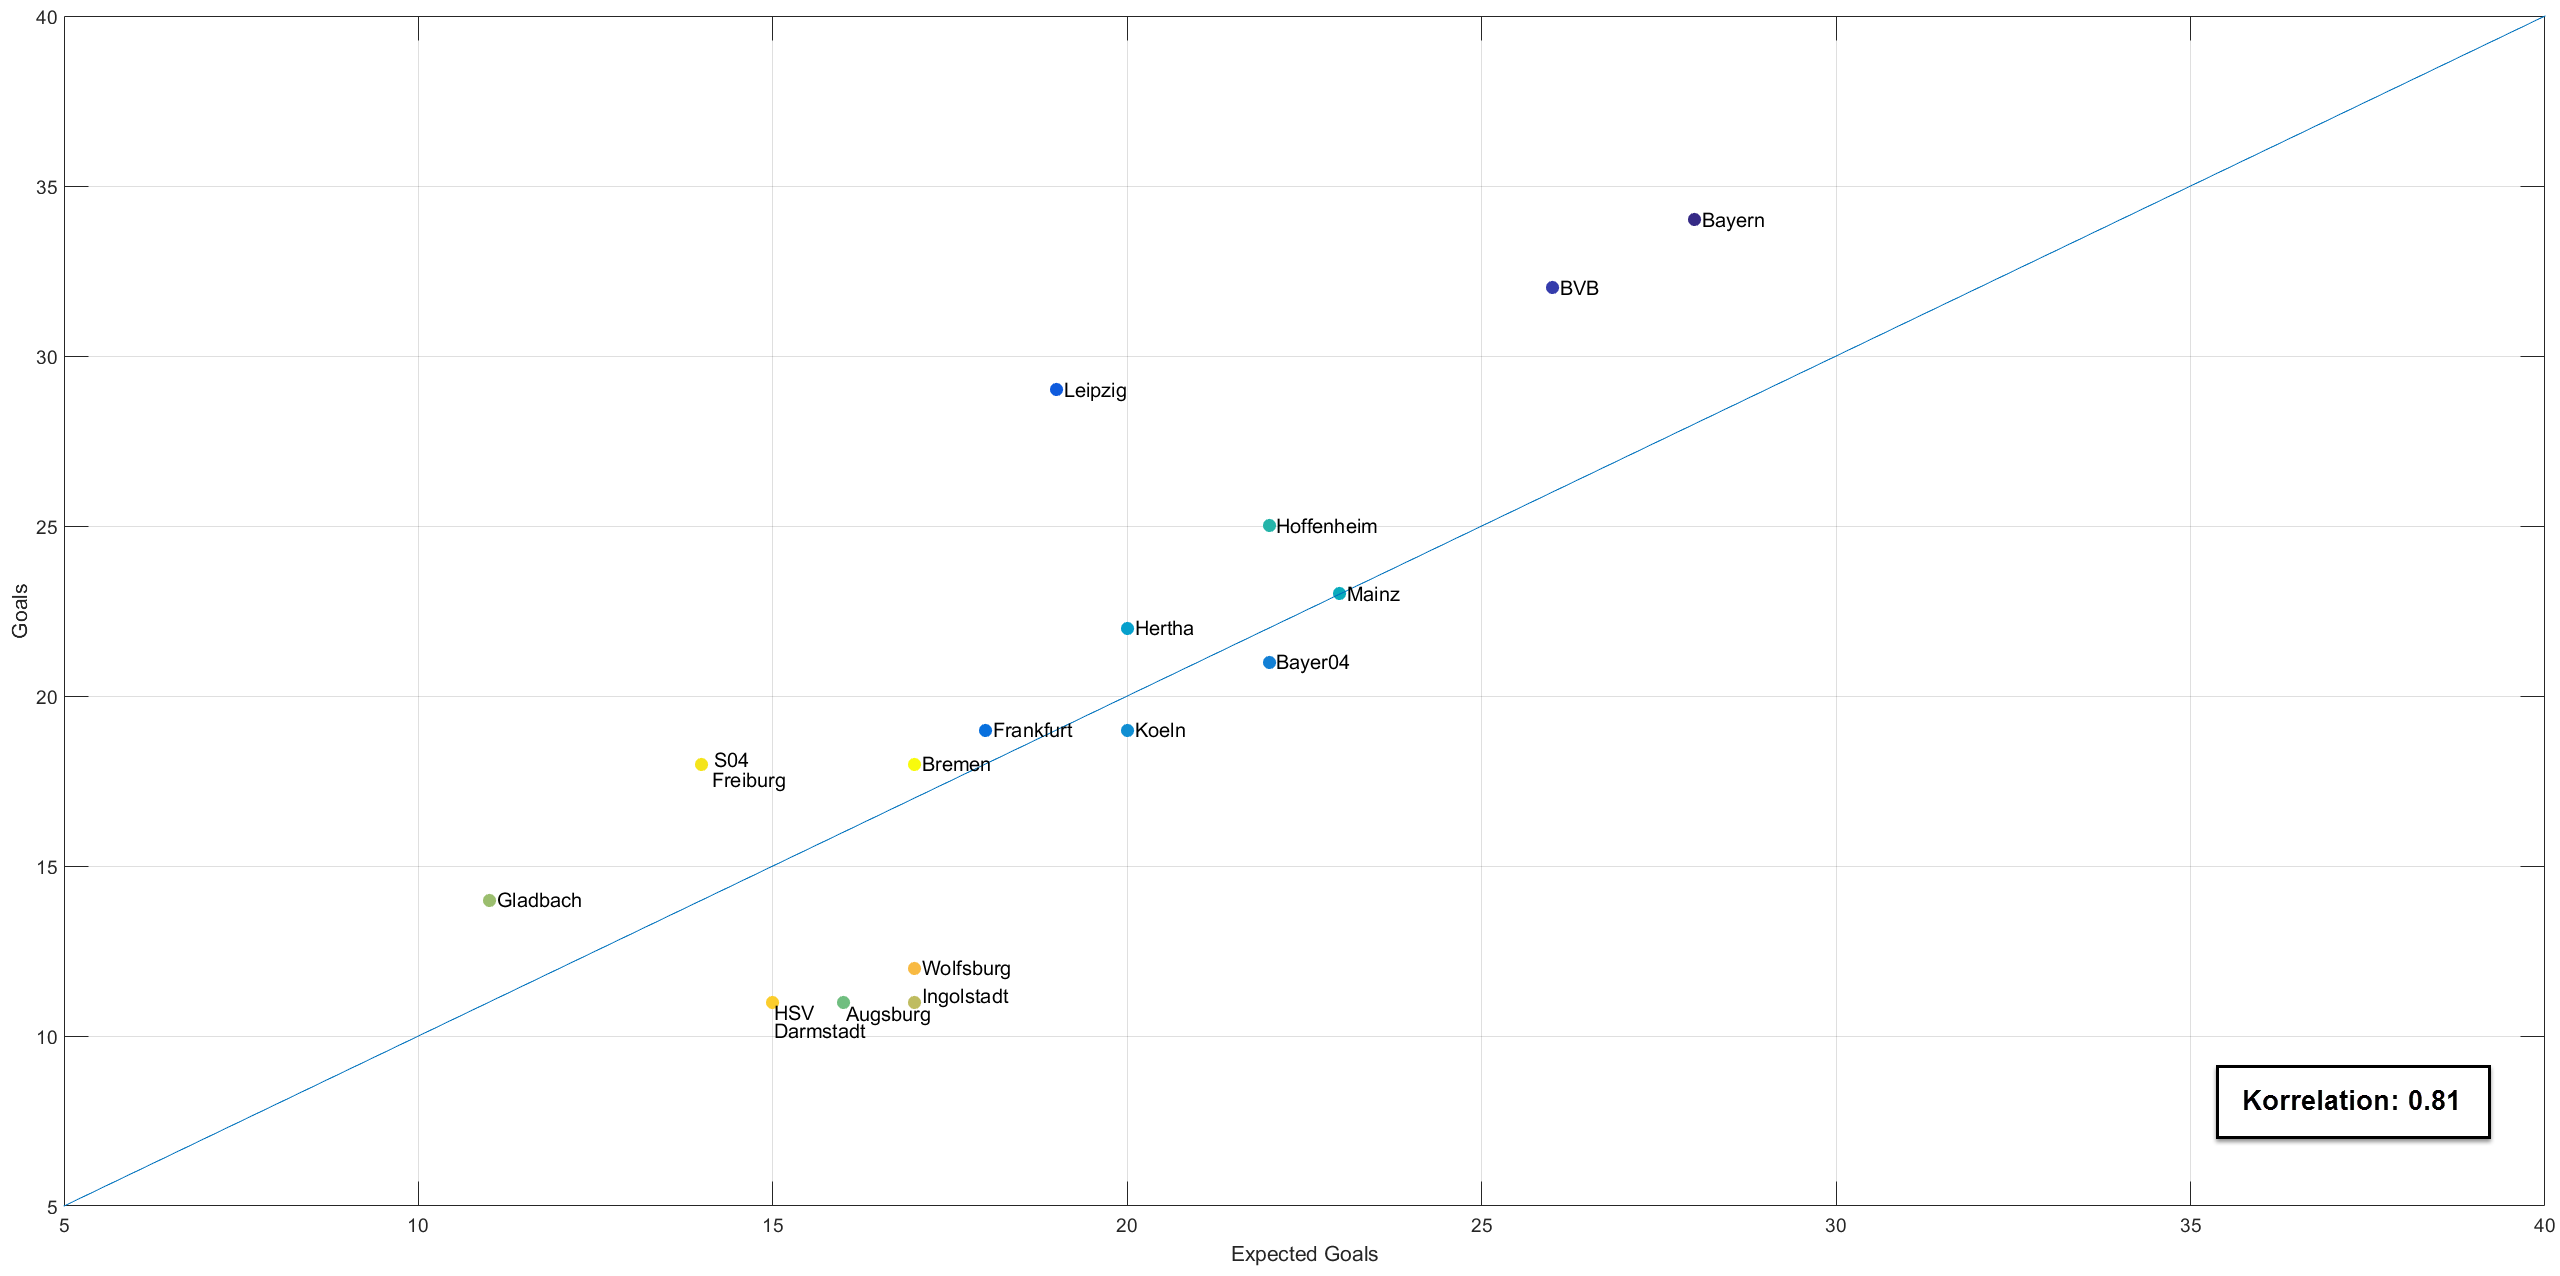
\includegraphics[scale=0.3]{se-wa-jpg/goals_correlation_16_17}
\caption{Evaluation der Tore der Saison 2016/17}
\label{lines}
\end{sidewaysfigure}

\begin{sidewaysfigure}
\centering
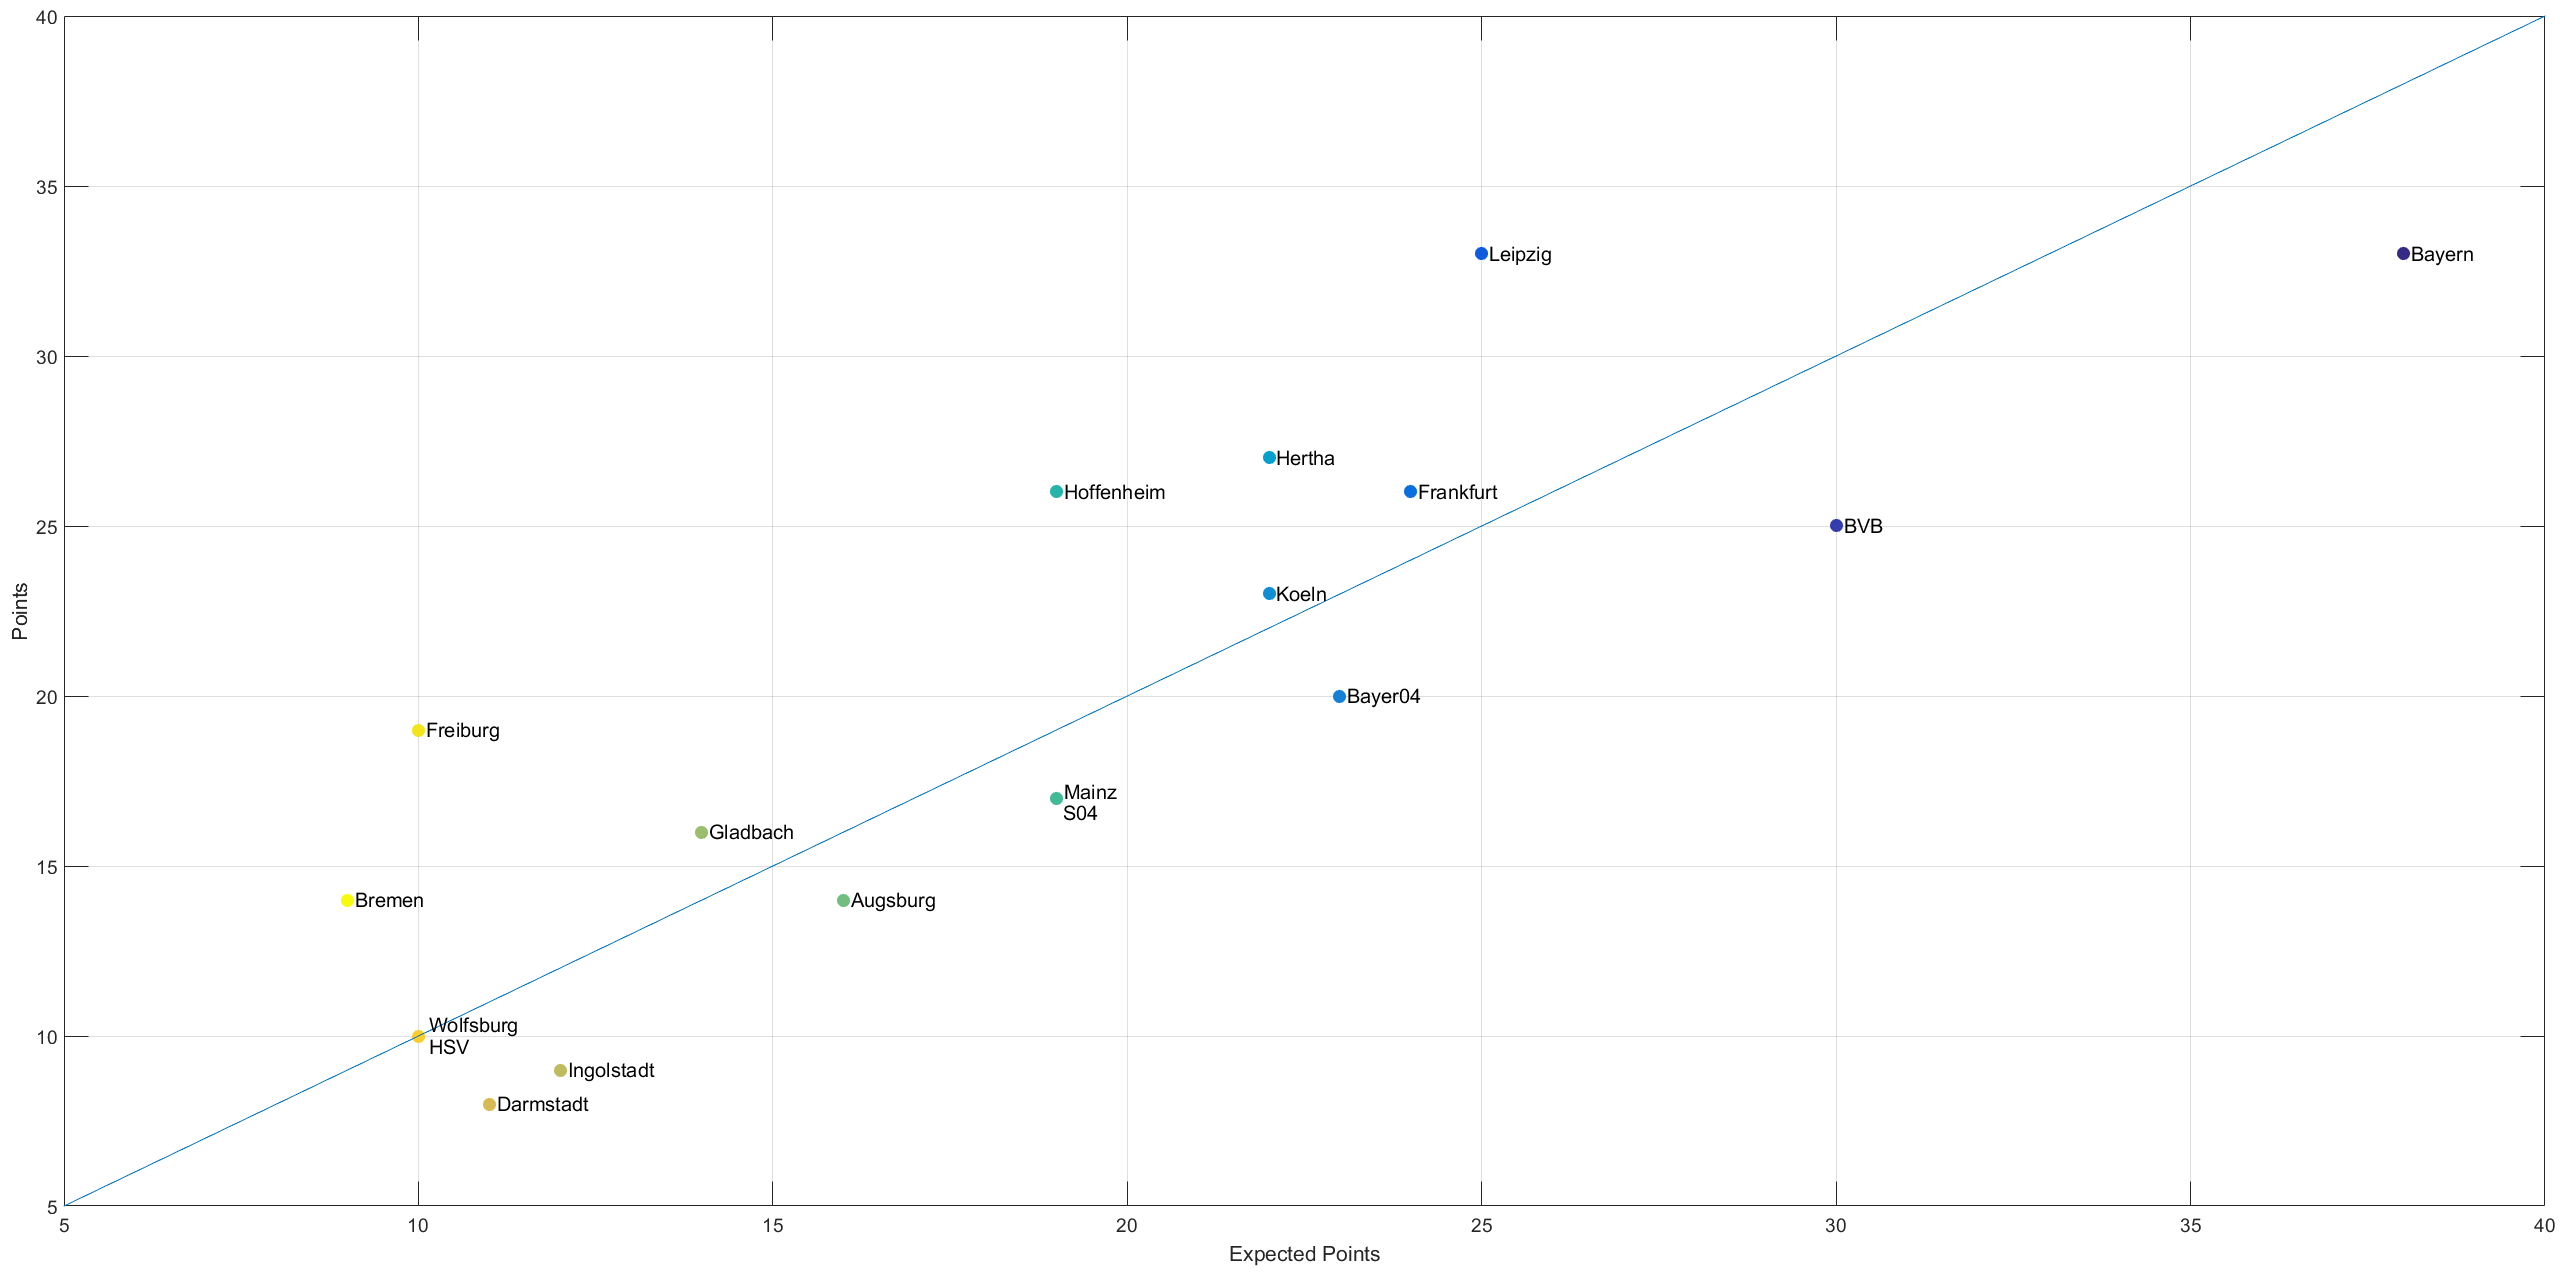
\includegraphics[scale=0.3]{se-wa-jpg/points_correlation_16_17}
\caption{Evaluation der Punkte der Saison 2016/17}
\label{lines}
\end{sidewaysfigure}



